%%%%%%%%%%%%%%%%%%%%%%%%%%%%%%%%%%%%%%%%%%%%%%%%%%%%%%%%%%%%%%%%%%%%%%%%%%%%%%%%
%% Plantilla de memoria en LaTeX para la ETSIT - Universidad Rey Juan Carlos
%%
%% Por Gregorio Robles <grex arroba gsyc.urjc.es>
%%     Grupo de Sistemas y Comunicaciones
%%     Escuela Técnica Superior de Ingenieros de Telecomunicación
%%     Universidad Rey Juan Carlos
%% (muchas ideas tomadas de Internet, colegas del GSyC, antiguos alumnos...
%%  etc. Muchas gracias a todos)
%%
%% La última versión de esta plantilla está siempre disponible en:
%%     https://github.com/gregoriorobles/plantilla-memoria
%%
%% Para obtener PDF, ejecuta en la shell:
%%   make
%% (las imágenes deben ir en PNG o JPG)

%%%%%%%%%%%%%%%%%%%%%%%%%%%%%%%%%%%%%%%%%%%%%%%%%%%%%%%%%%%%%%%%%%%%%%%%%%%%%%%%

\documentclass[a4paper, 12pt]{book}
%\usepackage[T1]{fontenc}

\usepackage[a4paper, left=2.5cm, right=2.5cm, top=3cm, bottom=3cm]{geometry}
\usepackage{times}
\usepackage[utf8]{inputenc}
\usepackage[spanish]{babel} % Comenta esta línea si tu memoria es en inglés
\usepackage{url}
%\usepackage[dvipdfm]{graphicx}
\usepackage{graphicx}
\usepackage{float}  %% H para posicionar figuras
\usepackage[nottoc, notlot, notlof, notindex]{tocbibind} %% Opciones de índice
\usepackage{latexsym}  %% Logo LaTeX

\title{Memoria del Proyecto}
\author{Nombre del autor}

\renewcommand{\baselinestretch}{1.5}  %% Interlineado

\begin{document}

\renewcommand{\refname}{Bibliografía}  %% Renombrando
\renewcommand{\appendixname}{Apéndice}

%%%%%%%%%%%%%%%%%%%%%%%%%%%%%%%%%%%%%%%%%%%%%%%%%%%%%%%%%%%%%%%%%%%%%%%%%%%%%%%%
% PORTADA

\begin{titlepage}
\begin{center}

\includegraphics[scale=0.8]{img/URJ_logo_Color_POS.png}

\vspace{1.75cm}

\Large
GRADO EN INGENIERÍA EN SISTEMAS AUDIOVISUALES Y MULTIMEDIA

\vspace{0.4cm}

\large
Curso Académico 2021/2022

\vspace{0.8cm}

Trabajo Fin de Grado

\vspace{2.5cm}

\LARGE
AMPLIACIÓN DEL ANÁLISIS DE CÓDIGO PYTHON CON CEFRL 

\vspace{4cm}

\large
Autor : Javier Jiménez Ramiro \\
Tutor : Dr. Gregorio Robles Martínez
\end{center}
\end{titlepage}

\newpage
\mbox{}
\thispagestyle{empty} % para que no se numere esta pagina


%%%%%%%%%%%%%%%%%%%%%%%%%%%%%%%%%%%%%%%%%%%%%%%%%%%%%%%%%%%%%%%%%%%%%%%%%%%%%%%%
%%%% Para firmar
\clearpage
\pagenumbering{gobble}
\chapter*{}

\vspace{-4cm}
\begin{center}
\LARGE
\textbf{Trabajo Fin de Grado}

\vspace{1cm}
\large
Ampliación del Análisis de Código Python con CEFRL

\vspace{1cm}
\large
\textbf{Autor :} Javier Jiménez Ramiro \\
\textbf{Tutor :} Dr. Gregorio Robles Martínez

\end{center}

\vspace{1cm}
La defensa del presente Proyecto Fin de Carrera se realizó el día \qquad$\;\,$ de \qquad\qquad\qquad\qquad \newline de 2022, siendo calificada por el siguiente tribunal:


\vspace{0.5cm}
\textbf{Presidente:}

\vspace{1.2cm}
\textbf{Secretario:}

\vspace{1.2cm}
\textbf{Vocal:}


\vspace{1.2cm}
y habiendo obtenido la siguiente calificación:

\vspace{1cm}
\textbf{Calificación:}


\vspace{1cm}
\begin{flushright}
Fuenlabrada, a \qquad$\;\,$ de \qquad\qquad\qquad\qquad de 2022
\end{flushright}

%%%%%%%%%%%%%%%%%%%%%%%%%%%%%%%%%%%%%%%%%%%%%%%%%%%%%%%%%%%%%%%%%%%%%%%%%%%%%%%%
%%%% Dedicatoria

\chapter*{}
\pagenumbering{Roman} % para comenzar la numeracion de paginas en numeros romanos
\begin{flushright}
\textit{Un alma saludable\\ habita en un cuerpo y una mente saludables.\\
Maka Albarn}
\end{flushright}

%%%%%%%%%%%%%%%%%%%%%%%%%%%%%%%%%%%%%%%%%%%%%%%%%%%%%%%%%%%%%%%%%%%%%%%%%%%%%%%%
%%%% Agradecimientos

\chapter*{Agradecimientos}
%\addcontentsline{toc}{chapter}{Agradecimientos} % si queremos que aparezca en el índice
\markboth{AGRADECIMIENTOS}{AGRADECIMIENTOS} % encabezado 

Con este proyecto doy final a una maravillosa etapa universitaria, un camino recorrido junto a mucha gente, gente que vino y se quedo, gente que siempre estuvo ahí y gente que se acabó yendo pero que aprendí algo de ellos.

Por ello quiero dar las gracias a esas personas que siempre estuvieron ahí y que creyeron en que yo podría conseguirlo. La primera de estas personas soy yo mismo, quiero agradecer el no rendirme nunca, el seguir luchando por muy difícil que se pusiera todo y el hecho de que si caía derrotado o cometía algún error me levantaba y lo solucionaba asumiendo las consecuencias necesarias.

Por supuesto agradecer a mis padres, porque ellos lucharon día a día para permitirme cumplir este sueño, me ayudaron y me apoyaron y a día de hoy lo siguen haciendo. Siempre recordaré los abrazos de mi madre y la frase que me dijo mi padre el primer día de esta etapa: ``si tienes algún problema estoy solo a tres horas de coche".

También me gustaría agradecer a mis dos hermanos, las dos personas que más me han escuchado y ayudado en los malos momentos, mi hermano de sangre y mi hermana de espíritu. Mi hermano me enseño que la etapa universitaria debes tomarla con calma, no amargarte y seguir luchando, me enseñó que si quieres algo debes luchar que nadie te lo regala y me enseñó que ser el mejor es cuestión de actitud y creer que puedes. Mi hermana me enseñó la importancia de la tranquilidad, me enseñó que puedo superar mis miedos y que soy mucho más de lo que creo, me escuchó siempre y siempre estuvo ahí cuando la necesité, lloró conmigo y rió conmigo y me enseñó que la paz vive en nuestro interior, que no eres ni más ni menos que nadie y que todos merecemos un abrazo, una sonrisa y mucho respeto. Y que si transmites alegría, recibes alegría.

Por último y no menos importante agradecerle a mi mano izquierda, el regalo que me dio la universidad y uno de mis mejores amigos, el hizo que estar a tres horas de mi hogar fuera más ameno. Darle las gracias a ellos y a mis profesores en especial a Susana que hizo que el inglés fuese divertido y a Gregorio que me ayudo a que este proyecto siguiera, me transmitió su pasión por Python y ayudó a que todo fuese más fácil. Gracias a todos.

%%%%%%%%%%%%%%%%%%%%%%%%%%%%%%%%%%%%%%%%%%%%%%%%%%%%%%%%%%%%%%%%%%%%%%%%%%%%%%%%
%%%% Resumen

\chapter*{Resumen}
%\addcontentsline{toc}{chapter}{Resumen} % si queremos que aparezca en el índice
\markboth{RESUMEN}{RESUMEN} % encabezado

El objetivo de este proyecto es ampliar la herramienta ya existente de análisis de código Python, inspirada en los niveles del CEFRL, con dos nuevas opciones de análisis como son fragmentos de respuestas en la web Stack Overflow y aportaciones a proyectos mediante Pull Request en GitHub, añadiendo filtros y adecuando los fragmentos de código al método de análisis ya existente.

El uso de esta herramienta está enfocado, ya no solo en la educación y evaluación del alumnado, en ser capaces de evaluar código externo para poder añadirlo a nuestros proyectos cerciorandonos de que el código es de buena calidad o está acorde a nuestro nivel de comprensión.

Para ello se han utilizado varias tecnologías. El lenguaje Python para la extracción del código como para el desarrollo de los filtros, JSON para la muestra de resultados y tanto GitHub como Stack Overflow para la obtención de ejemplos y pruebas y para la base de desarrollo de este proyecto.

%%%%%%%%%%%%%%%%%%%%%%%%%%%%%%%%%%%%%%%%%%%%%%%%%%%%%%%%%%%%%%%%%%%%%%%%%%%%%%%%
%%%% Resumen en inglés

\chapter*{Summary}
%\addcontentsline{toc}{chapter}{Summary} % si queremos que aparezca en el índice
\markboth{SUMMARY}{SUMMARY} % encabezado

The objective of this project is to extend the existing Python code analysis tool, inspired by the CEFRL levels, with two new analysis options such as response snippets on the Stack Overflow website and contributions to projects via Pull Request on GitHub, adding filters and adapting the code snippets to the existing analysis method.

The use of this tool is focused, not only in the education and evaluation of students, in being able to evaluate external code to be able to add it to our projects making sure that the code is of good quality or is according to our level of understanding.

Several technologies have been used for this purpose. The Python language for code extraction and filter development, JSON for sample results and both GitHub and Stack Overflow for obtaining examples and tests and for the development base of this project.


%%%%%%%%%%%%%%%%%%%%%%%%%%%%%%%%%%%%%%%%%%%%%%%%%%%%%%%%%%%%%%%%%%%%%%%%%%%%%%%%
%%%%%%%%%%%%%%%%%%%%%%%%%%%%%%%%%%%%%%%%%%%%%%%%%%%%%%%%%%%%%%%%%%%%%%%%%%%%%%%%
% ÍNDICES %
%%%%%%%%%%%%%%%%%%%%%%%%%%%%%%%%%%%%%%%%%%%%%%%%%%%%%%%%%%%%%%%%%%%%%%%%%%%%%%%%

% Las buenas noticias es que los índices se generan automáticamente.
% Lo único que tienes que hacer es elegir cuáles quieren que se generen,
% y comentar/descomentar esa instrucción de LaTeX.

%%%% Índice de contenidos
\tableofcontents 
%%%% Índice de figuras
\cleardoublepage
%\addcontentsline{toc}{chapter}{Lista de figuras} % para que aparezca en el indice de contenidos
\listoffigures % indice de figuras
%%%% Índice de tablas
%\cleardoublepage
%\addcontentsline{toc}{chapter}{Lista de tablas} % para que aparezca en el indice de contenidos
%\listoftables % indice de tablas


%%%%%%%%%%%%%%%%%%%%%%%%%%%%%%%%%%%%%%%%%%%%%%%%%%%%%%%%%%%%%%%%%%%%%%%%%%%%%%%%
%%%%%%%%%%%%%%%%%%%%%%%%%%%%%%%%%%%%%%%%%%%%%%%%%%%%%%%%%%%%%%%%%%%%%%%%%%%%%%%%
% INTRODUCCIÓN %
%%%%%%%%%%%%%%%%%%%%%%%%%%%%%%%%%%%%%%%%%%%%%%%%%%%%%%%%%%%%%%%%%%%%%%%%%%%%%%%%

\cleardoublepage
\chapter{Introducción}
\label{sec:intro} % etiqueta para poder referenciar luego en el texto con ~\ref{sec:intro}
\pagenumbering{arabic} % para empezar la numeración de página con números

En el mundo de auge tecnológico en el que vivimos, en el que cada año muchas de las tecnologías se quedan obsoletas por el nacimiento o desarrollo de otras, la forma más rápida y fácil de crecer y ampliar el conocimiento es compartiéndolo con otras personas, es decir, intercambiando ideas y trabajando en equipo.

Como desarrollador software tienes dos maneras principales de hacer esto, o bien preguntando a una comunidad de miles de personas con más experiencia y conocimientos que puedan aportarte una solución práctica a tu problema, o bien permitiendo el hecho de que otros desarrolladores puedan darte consejos y mejoras a tu proyecto dejando todo tu código fuente a disposición de todo el mundo que quiera aportar altruistamente su granito de arena.

Esto se puede realizar por medio de páginas web con comunidades de dimensiones mundiales como github\footnote{https://github.com/} o stackoverflow\footnote{https://stackoverflow.com/}.

Pero, al tener acceso todo el mundo, ¿Cómo podemos saber si una respuesta o una aportación es correcta? Y profundizando más aún, ¿Cómo podemos saber si esa misma respuesta o aportación tiene el nivel que nosotros deseamos para nuestro proyecto?.

Pues así nació la idea de este proyecto, el poder analizar las respuestas dadas en stackoverflow y las aportaciones ofrecidas en github por medio del uso del software de un proyecto anterior centrándonos en el lenguaje de programación de código abierto Python.

Aunque realmente la idea del inicio de este proyecto va aun mas profundo, pues lo que realmente motiva la creación de este proyecto es el poder aumentar la calidad de las interacciones de los usuarios, clasificar las respuestas o las aportaciones de cada usuario a cualquier proyecto sabiendo si de verdad están haciendo una gran aportación e incluso sabiendo que usuarios hacen las mejores aportaciones consiguiendo así cada vez más calidad en la ayuda ofrecido y pudiendo elegir que aportaciones queremos añadir a nuestros proyectos porque de verdad hacen nuestro código de mayor calidad pudiendo llegar a ser una comunidad cada vez más eficiente y con mayor calidad en los proyectos que estén por venir. Por ejemplo, imaginemos un proyecto alojado en un repositorio en GitHub que recibe una gran cantidad de aportaciones o Pull Request diarias, si nosotros como creadores de ese proyecto tuviéramos que mirar con lupa cada una de estas aportaciones no acabaríamos nunca y lo que es peor estaríamos perdiendo mucho tiempo y por lo tanto haciendo que nuestro proyecto avance muy lentamente, pero gracias a la herramienta creada en este proyecto podríamos. de una manera rápida y eficiente, añadir las mejores aportaciones a nuestro proyecto haciendo que este tenga una mayor calidad y crezca mucho más rápido, lo mismo pasa en Stack Overflow, si añadimos una pregunta y recibimos una gran cantidad de respuestas con esta herramienta podemos probar antes aquellas que tengan una mayor calidad encontrando la solución a nuestro problema de manera mucho más rápida.

Este proyecto mencionado en el párrafo anterior ya era útil para conocer cual es tu nivel en python, ver tu propia mejoría o incluso en el ámbito de la educación poder analizar y evaluar los proyectos del alumnado haciendo más fácil y rápida esta tarea, pero gracias a esta ampliación ahora también podrás ver que aportaciones o que respuestas son las más adecuadas para cada uno de tus proyectos mediante el marco e análisis, ya utilizado en muchos campos, CEFRL.

Este marco nos permite el dividir en tres categorías con dos subcategorías cada una, estas categorías son: usuario básico (A), usuario independiente (B) y usuario competente (C).

Así por este método, aunque el lema de python sea ``solo hay una manera de hacer las cosas", podremos reescribir este lema diciendo ``hay maneras más correctas que otras de hacer la cosas" y escoger por nosotros mismos las que más se adecuen a nuestro proyecto y entendimiento.

\section{Estructura de la memoria}
\label{sec:estructura}

En cuanto a la estructura, se divide está memoria en 7 grandes capítulos abordando cada una de las cuestiones más importante de este proyecto.

Los capítulos son:

\begin{itemize}
  \item \textbf{Capítulo 1:} En este capítulo se muestra la introducción del proyecto y la estructura que llevará la memoria al completo.
  
  \item \textbf{Capítulo 2:} En este capítulo se abordan los objetivos tanto generales como específicos que se han seguido para el desarrollo del proyecto así como una planificación temporal el mismo.
  
  \item \textbf{Capítulo 3:} En este capítulo se desarrolla una breve explicación de todas las tecnologías usadas en la realización del proyecto.
  
  \item \textbf{Capítulo 4:} En este capítulo se muestra todo el proceso que se ha llevado a cabo para completar la ampliación del análisis de código Python de manera detallada.
  
  \item \textbf{Capítulo 5:}
  
  \item \textbf{Capítulo 6:}
  
  \item \textbf{Capítulo 7:} En este capítulo se abordan todos los problemas y éxitos encontrados a la hora de realizar los objetivos mencionados en el capítulo 2, todo lo aplicado y aprendido durante el desarrollo del grado de manera personal y posibles trabajos futuros que ayuden a la mejora constante de esta herramienta.
\end{itemize}



%%%%%%%%%%%%%%%%%%%%%%%%%%%%%%%%%%%%%%%%%%%%%%%%%%%%%%%%%%%%%%%%%%%%%%%%%%%%%%%%
%%%%%%%%%%%%%%%%%%%%%%%%%%%%%%%%%%%%%%%%%%%%%%%%%%%%%%%%%%%%%%%%%%%%%%%%%%%%%%%%
% OBJETIVOS %
%%%%%%%%%%%%%%%%%%%%%%%%%%%%%%%%%%%%%%%%%%%%%%%%%%%%%%%%%%%%%%%%%%%%%%%%%%%%%%%%

\cleardoublepage % empezamos en página impar
\chapter{Objetivos} % título del capítulo (se muestra)
\label{chap:objetivos} % identificador del capítulo (no se muestra, es para poder referenciarlo)

\section{Objetivo general} % título de sección (se muestra)
\label{sec:objetivo-general} % identificador de sección (no se muestra, es para poder referenciarla)

Mi trabajo de fin de grado consiste en ampliar las opciones de análisis de la herramienta software de evaluación de código python, version 3, inspirada en el marco CEFRL con el análisis de las respuestas dadas en stackoverflow y las aportaciones dadas en github a través de pull requests. 

Con esto seremos capaces de introducir esta ayuda externa en nuestro código sabiendo exactamente cómo de buenas son estas aportaciones.


\section{Objetivos específicos}
\label{sec:objetivos-especificos}

Para el objetivo general descrito anteriormente se han de abordar los siguientes objetivos específicos:

\begin{itemize}
	\item Estudiar y entender el funcionamiento de análisis ya existente dentro del programa de pycefrl y comprobar la funcionalidad ya instalada siguiendo los pasos dentro del código.
	\item Modificar y añadir las funcionalidades nuevas descritas anteriormente acondicionandolas e integrandolas para su correcto paso por el análisis del programa.
	\item Extraer y guardar los fragmentos de código útiles para su futuro análisis.
	\item estudiar y aplicar los diferentes filtros para cada una de las nuevas funcionalidades y poder transformar el fragmento de código en un objeto útil para su análisis.
	\item probar las nuevas funcionalidades con cien URLs de interés para cada opción.
	\item Mejorar dentro de lo posible aquellos fallos que muestren los distintos filtros después de la primera batería de pruebas.
	\item Probar de nuevo y anotar todos los resultados para cada opción para poder cerciorarnos de la eficacia del análisis y de las condiciones para que el mismo sea correcto. 
\end{itemize}


\section{Planificación temporal}
\label{sec:planificacion-temporal}

Este proyecto comenzó en febrero de 2022, después de un intento fallido de TFG que comenzó en septiembre del año anterior.

Después de trabajar en el primer intento ocurrió un error en enero de 2022 que dejó mi ordenador inservible y supuso la perdida de todos los datos y de todo el trabajo de esos meses, lo que causo que, tras mucho valorar, decidí que necesitaba un cambio a otro proyecto que llamase mucho más mi interés.

Y así, teniendo claro que yo quería que tratase sobre programación y aún más importante sobre Python, comencé con este proyecto con muchas más fuerzas e ilusión.

En los primeros dos meses de trabajo, febrero y marzo, se consiguió la correcta extracción de los fragmentos de código de interés pero sin tener éxito en el resultado final de su análisis, creyendo que era por culpa del análisis se decidió abordar la parte analítica y comprobar que podía estar fallando, esto costó mucho tiempo ya que a la vez que trabajaba en este proyecto la mitad de la tarde de lunes a viernes, al rededor de dos horas y media al día, también trabajaba en las prácticas por las mañanas y estudiaba para obtener el titulo B1 de inglés asistiendo al final de la tarde a una academia.

Tras estos dos meses a mediados de abril, después de una reunión de dudas con mi tutor, me di cuenta que realmente el fallo no se encontraba en el análisis si no en los filtros utilizados para el acondicionamiento del fragmento de código a analizar, por lo tanto, pasé el resto abril dedicando la tarde completa y las primeras semanas de mayo dedicando toda la mañana ya que había finalizado mis prácticas de empresa, al rededor de 5 horas por día de lunes a jueves, a mejorar y añadir los filtros que consideraba necesarios y útiles.

El resto del mes de mayo y parte de la primera semana de junio durante toda la mañana de lunes a jueves, habiendo terminado todos los filtros, me dediqué a probar mi herramienta con cien URLs por opción, doscientas en total, y anotando los resultados y porcentajes.

Por último la segunda semana de Junio se comenzó con la memoria con vistas a entregarla en el mismo mes y realizar su defensa a principios del mes de julio. 


%%%%%%%%%%%%%%%%%%%%%%%%%%%%%%%%%%%%%%%%%%%%%%%%%%%%%%%%%%%%%%%%%%%%%%%%%%%%%%%%
%%%%%%%%%%%%%%%%%%%%%%%%%%%%%%%%%%%%%%%%%%%%%%%%%%%%%%%%%%%%%%%%%%%%%%%%%%%%%%%%
% ESTADO DEL ARTE %
%%%%%%%%%%%%%%%%%%%%%%%%%%%%%%%%%%%%%%%%%%%%%%%%%%%%%%%%%%%%%%%%%%%%%%%%%%%%%%%%

\cleardoublepage
\chapter{Estado del arte}
\label{chap:estado}

En este capitulo se explican las tecnologías más importantes utilizadas en el desarrollo de este proyecto.

\section{Python}
\label{sec:Python}

Python~\cite{website:Python} es un lenguaje de programación de alto nivel, interpretado y de propósito general. Su filosofía de diseño enfatiza la legibilidad del código con el uso de una sangría significativa. A menudo se describe como un lenguaje ``con pilas incluidas" debido a su completa biblioteca estándar. 

En cuanto a su historia, Python fue concebido a finales de la década de 1980 por Guido van Rossum en el Centrum Wiskunde Informatica de los Países Bajos como sucesor del lenguaje de programación ABC, inspirado en SETL, capaz de manejar excepciones y de interactuar con el sistema operativo Amoeba. Su implementación comenzó en diciembre de 1989. Python 3.0, publicado el 3 de diciembre de 2008, con muchas de sus principales características retrocedidas a Python 2.6.x y 2.7.x. Las versiones de Python 3 incluyen la utilidad 2to3, que automatiza la traducción del código de Python 2 a Python 3.
Posteriormente, también se dejó de dar soporte a la versión 3.6. En 2021, Python 3.9.2 y 3.8.8 fueron acelerados ya que todas las versiones de Python tenían problemas de seguridad que conducían a una posible ejecución remota de código y envenenamiento de la caché web.

En su diseño, Python es un lenguaje de programación multiparadigma. La programación orientada a objetos y la programación estructurada están totalmente soportadas, y muchas de sus características soportan la programación funcional y la programación orientada a aspectos. Muchos otros paradigmas están soportados a través de extensiones, incluyendo el diseño por contrato y la programación lógica. Su diseño ofrece cierto apoyo a la programación funcional en la tradición Lisp.

Las normas de su filosofía mas destacadas son:

\begin{itemize}
	\item Bonito mejor que feo.
	\item Explicito es mejor que implícito.
	\item Lo simple mejor que lo complejo.
	\item Lo complejo es mejor que lo complicado.
	\item La legibilidad cuenta.
\end{itemize}

En lugar de construir toda su funcionalidad en su núcleo, Python fue diseñado para ser altamente extensible a través de módulos. Python se esfuerza por conseguir una sintaxis y una gramática más sencillas y menos recargadas, al tiempo que ofrece a los desarrolladores la posibilidad de elegir su metodología de codificación. Los desarrolladores de Python se esfuerzan por evitar la optimización prematura y rechazan los parches en partes no críticas de la implementación de referencia de CPython que ofrecerían incrementos marginales de velocidad a costa de la claridad.
Un neologismo común en la comunidad de Python es pitónico, que tiene una amplia gama de significados relacionados con el estilo del programa.


\section{JSON}
\label{sec:JSON}

JSON~\cite{website:JSON} es un formato de texto sencillo para el intercambio de datos. Una de las supuestas ventajas de JSON sobre XML como formato de intercambio de datos es que resulta mucho más sencillo escribir un analizador sintáctico para él. Por esa razón, JSON se emplea habitualmente en entornos donde el tamaño del flujo de datos entre cliente y servidor es de vital importancia cuando la fuente de datos es explícitamente de fiar y donde no es importante el hecho de no disponer de procesamiento XSLT para manipular los datos en el cliente.

Un ejemplo de datos JSON podría ser:
{\footnotesize
\begin{verbatim}
{
  "departamento":8,
  "nombredepto":"Ventas",
  "director": "Juan Rodríguez",
  "empleados":[
    {
      "nombre":"Pedro",
      "apellido":"Fernández"
    },{
      "nombre":"Jacinto",
      "apellido":"Benavente"
    } 
  ]
}
\end{verbatim}
}

\section{Github}
\label{sec:Github}

GitHub~\cite{website:GitHub} es una forja(plataforma de desarrollo colaborativo) para alojar proyectos utilizando el sistema de control de versiones Git. El software que opera GitHub fue escrito en Ruby on Rails. El código de los proyectos alojados en GitHub se almacena generalmente de forma pública.

\subsection{Repositorios}

Los repositorios son, como su propio nombre indica, lugares virtuales alojados en la nube en donde los usuarios pueden almacenar cualquier tipo de archivo. Para ser identificados, los repositorios muestran información relevante, como la descripción del proyecto, los lenguajes de programación usados o las etiquetas de búsqueda. Un aspecto muy importante de la información de los repositorios es el archivo «README», el cual los desarrolladores pueden crear para describir su proyecto a fondo.

\subsection{Issues}

En GitHub, los Issues son abiertos por usuarios que tienen un fallo con el código del repositorio y quieren recibir ayuda para solucionarlo, pos usuarios que quieren plantear una compleja mejora del programa, entre otros usos. Se pueden enlazar pull requests a los issues, así como asignar usuarios y etiquestas.

\subsection{Pull Requests}

Las pull requests son solicitudes de admisión de código. Los usuarios pueden editar cualquier archivo de código de un repositorio, ya sea a través del editor integrado de GitHub o desde su ambiente local. Adicionalmente, pueden revisar el código y enviar comentarios a modo de retroalimentación. Este proceso se conoce como ``revisión de código".

\subsection{Debates}
Son parecidos a los Issues ya que pueden crearse sobre temas específicos y almacenar comentarios de otros usuarios a modo de foro. Para una mejor organización, los debates pueden clasificarse en diferentes categorías que el dueño del repositorio puede crear. A diferencia de los issues, hay un sistema de votos para los comentarios y un usuario con permisos en el repositorio puede marcar una respuesta como `correcta'. Pueden convertirse en issues.

\subsection{Acciones}

Es un servicio que permite al usuario crear flujos de trabajo con los cuales automatizar ciertas acciones, logrando así una integración continua y una entrega continua. Las acciones pueden ser personalizadas gracias al uso de archivos en un formato concreto.

\subsection{Wiki}

Una función muy útil para algunos repositorios es la de la creación de páginas de wiki. Gracias a estas, los creadores de los proyectos pueden escribir artículos que expliquen más cosas acerca del proyecto o de su funcionamiento.

\section{Stack Overflow}
\label{Stack Overflow}

Stack Overflow~\cite{website:StackOverflow} es un sitio de preguntas y respuestas para programadores profesionales y aficionados. Es el sitio emblemático de la red Stack Exchange, creado en 2008 por Jeff Atwood y Joel Spolsky. Contiene preguntas y respuestas sobre una amplia gama de temas de programación. Se creó para ser una alternativa más abierta a sitios previos de preguntas y respuestas como Experts-Exchange.

El funcionamiento de su web es bastante sencillo:
\begin{enumerate}
	\item El usuario se registra en la web
	\item El usuario realiza su pregunta y la hace pública
	\item El usuario comienza a recibir respuestas de la comunidad
\end{enumerate}

Las respuestas son publicadas por los miembros de una comunidad determinada o por otros usuarios con las mismas experiencias que encontraron solución al problema planteado.

Se ha convertido en una web muy fiable por diversas razones de las cuales se pueden destacar:

\begin{itemize}
	\item Confianza de los usuarios
	\item Habilidades de comunicación
	\item Calidad y relevancia en preguntas y respuestas
	\item Manejo de los temas
	\item Nivel de experiencia y participación
\end{itemize}

\section{Proyecto de programación del CEFRL}
\label{Proyecto de programación del CEFRL}

Este proyecto proporciona una tabla la cual evalúa las habilidades de programación de un usuario en tres clases, escritura, entendimiento e interacción, y a su vez en varias subclases como pueden ser reutilización del código o autoaprendizaje dentro del lenguaje.

Dependiendo del nivel adquirido en cada una de estas clases podemos catalogar a los programadores en tres grandes niveles divididos a su vez en dos niveles cada uno: 

\begin{itemize}
	\item A (A1, A2): el primer nivel sería para usuarios básicos capaces de realizar las tareas con guías o supervisión de programadores con niveles más altos.
	\item B (B1, B2): el segundo nivel sería para aquellos programadores prácticamente independientes que solo necesitarían de pequeñas orientaciones o indicaciones par realizar la tarea.
	\item C (C1, C2): el último nivel está reservado para todos aquellos programadores con nivel suficiente para no necesitar ninguna indicación y ser totalmente independientes.
\end{itemize}

Esta clasificación por niveles nos da mucha libertad a la hora de usarla ya que con ella podemos clasificar la dificultad de las diferentes tareas, la calidad de los proyectos e incluso evaluar las habilidades de un grupo de alumnos en cada clase y así también ser más eficientes a la hora de asignar trabajos y manejar equipos de la forma más correcta.

\section{Pycefr}
\label{Pycefr}

Esta herramienta es de la que se hace uso para realizar el análisis además de ser la base de mi proyecto. Por lo tanto en esta sección se explica como funciona la herramienta, de que hace uso y un ejemplo del resultado que ofrece.

Para comenzar la primera versión de la herramienta nos ofrecía un fichero de configuración, mencionado en capítulos posteriores, que nos permitía la personalización de niveles de los elementos de Python y sus variaciones creando así un diccionario que se utilizará en el análisis para la asignación del nivel (A1, A2, B1, B2, C1, C2) a cada fichero.

Una vez que se tiene este diccionario configurado se puede pasar a explicar la obtención de ficheros, para esta versión de la herramienta existen 3 opciones e infinitos valores. Las tres opciones son:

\begin{itemize}
	\item Directorio: el cual hace referencia a una carpeta local, por lo tanto el valor debe ser una ruta hacia esa carpeta.
	\item Repositorio: el cual hace referencia un proyecto alojado en GitHub, por lo tanto el valor debe ser una URL hacia ese repositorio.
	\item Usuario: el cual hacer referencia a un usuario de GitHub, por lo tanto el valor debe ser el nombre del usuario en cuestión.
\end{itemize}

Estas distintas opciones se explican detalladamente en capítulos posteriores. Sabiendo como se obtienen los ficheros podemos pasar a explicar el análisis en el cual se hace uso de la librería de Python ast\footnote{https://docs.python.org/3/library/ast.html}. Esta librería únicamente puede manejar Python3 ya que respecto a las versiones anteriores de Python la sintaxis del código ha cambiado.

Con el módulo ast se obtiene como resultado un arból de sintaxis abstracta utilizando el ayudante parse(). Para ello primero debemos definir las clases que nos interesan analizar del código Python como vemos en la figura \ref{fig:ast1} y \ref{fig:ast2}.


\begin{figure}
  \centering
  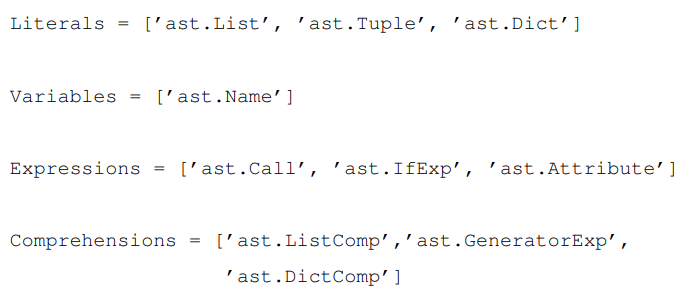
\includegraphics[width=9cm, keepaspectratio]{img/ast1.png}
  \caption{clases ast 1.}\label{fig:ast1}
\end{figure}

\begin{figure}
  \centering
  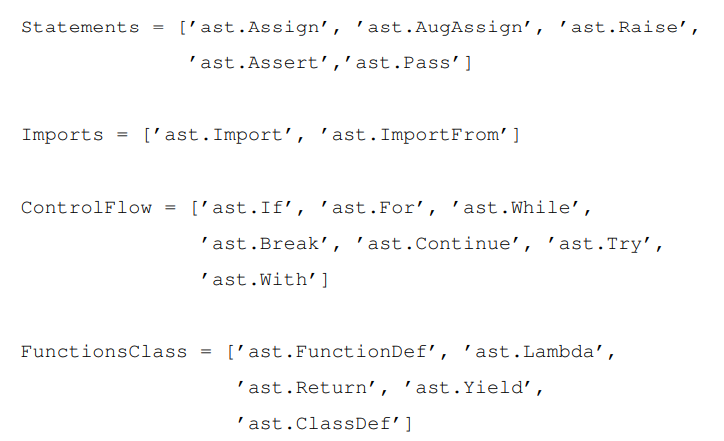
\includegraphics[width=9cm, keepaspectratio]{img/ast2.png}
  \caption{clases ast 2.}\label{fig:ast2}
\end{figure}

Gracias a esto aparecerá la clase IterTree, generando objetos compuestos por:

\begin{itemize}
	\item tree: es el árbol creado del repositorio o directorio donde se encuentra.
	\item attrib: es la clase del modulo ast.
	\item file: es el nombre del fichero más .py.
	\item repo: es el nombre de la carpeta a analizar.
\end{itemize}

después se empieza a recorrer cada nodo mediante el método ast.walk() comprobando los elementos dentro del nodo si corresponde a algunas de las clases mencionadas anteriormente mediante el programa levels.py, y se añadirá según el elemento la clase y el nivel correspondiente, extraído del diccionario mencionado anteriormente.

Por último, con las clases y niveles de antes, se crean los ficheros JSON y CSV. Dentro de estos ficheros aparecerá: el nombre del repositorio, el nombre del fichero, la clase del elemento, la línea donde empieza, la línea donde acaba, el desplazamiento de columna y el nivel del elemento.

Como resultado y centrando la atención en los archivos JSON obtenemos tres archivos distintos: el archivo JSON de cada repositorio encargado de almacenar los niveles y las clases y el número de apariciones de cada una de esta, el archivo JSON de todos los repositorios con la mima estructura que el anterior y un archivo JSON resumen de todos los repositorios donde se almacena un resumen de las clases y de los niveles totales. Estos archivos serán útiles para elaborar una página web de forma que se puedan ver los resultados de manera más gráfica.

\subsection{Ejemplo de uso}

En esta sección, como vemos en las figuras \ref{fig:ana1}, \ref{fig:ana2}, \ref{fig:ana3}, \ref{fig:ana4}, \ref{fig:ana5},  , muestro un ejemplo de uso de la herramienta explicada utilizando un repositorio de su creadora Ana Poveda Gracía Herrero.

\begin{figure}
  \centering
  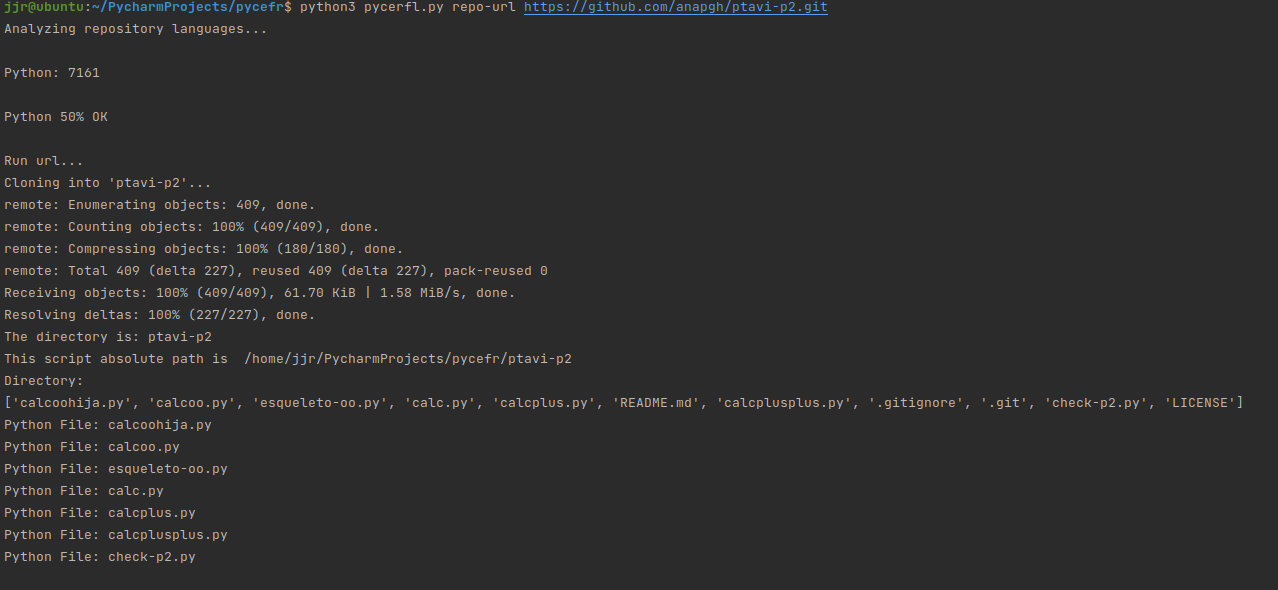
\includegraphics[width=1\textwidth]{img/ejemplousoana1.png}
  \caption{Ejemplo de ejecución.}\label{fig:ana1}
\end{figure}

\begin{figure}
  \centering
  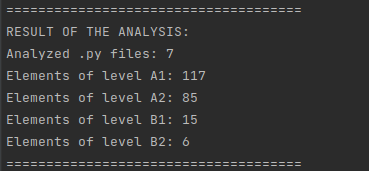
\includegraphics[width=9cm, keepaspectratio]{img/ejemplousoana2.png}
  \caption{Resultado de análisis.}\label{fig:ana2}
\end{figure}

\begin{figure}
  \centering
  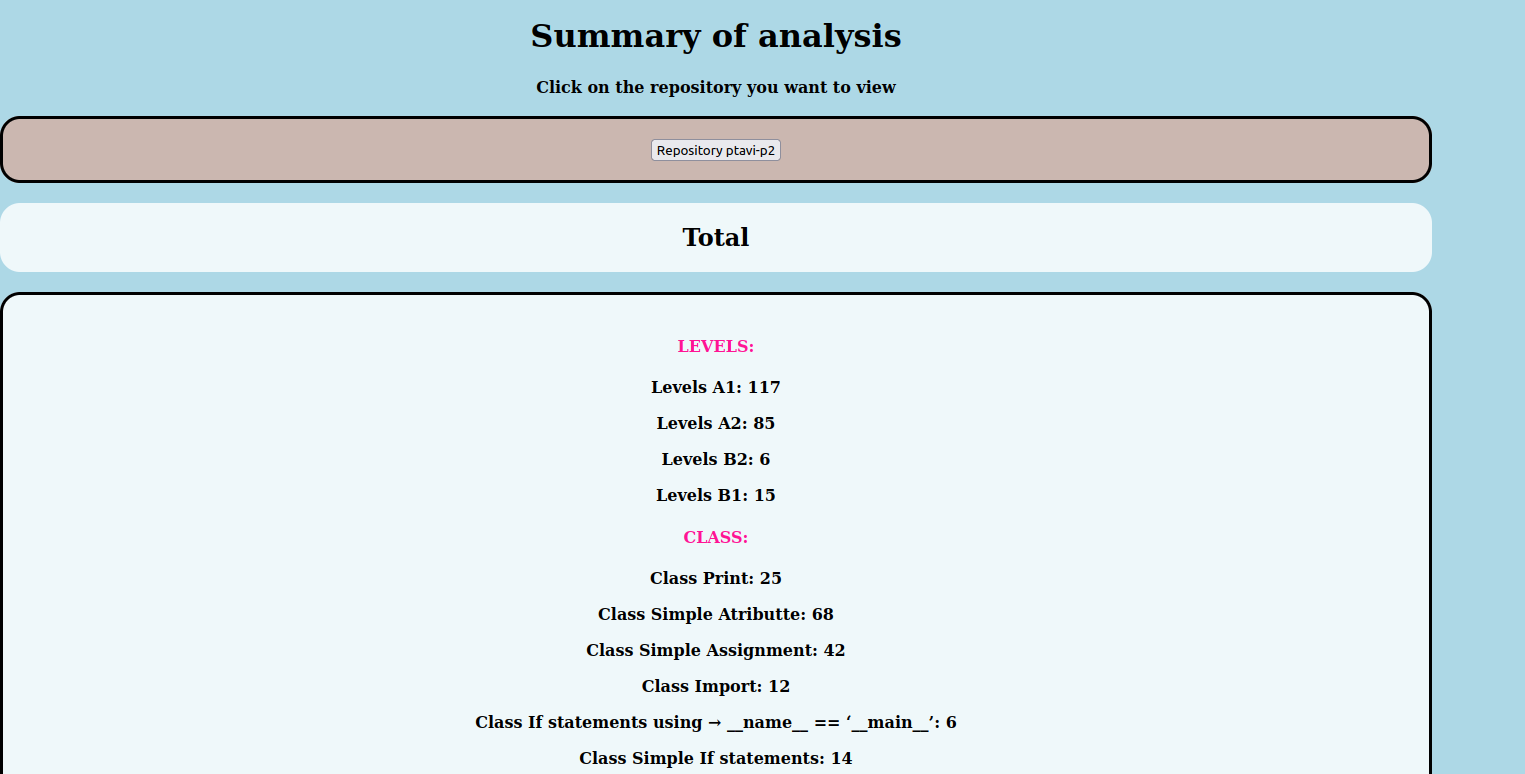
\includegraphics[width=1\textwidth]{img/ejemplousoana3.png}
  \caption{Página web principal.}\label{fig:ana3}
\end{figure}

\begin{figure}
  \centering
  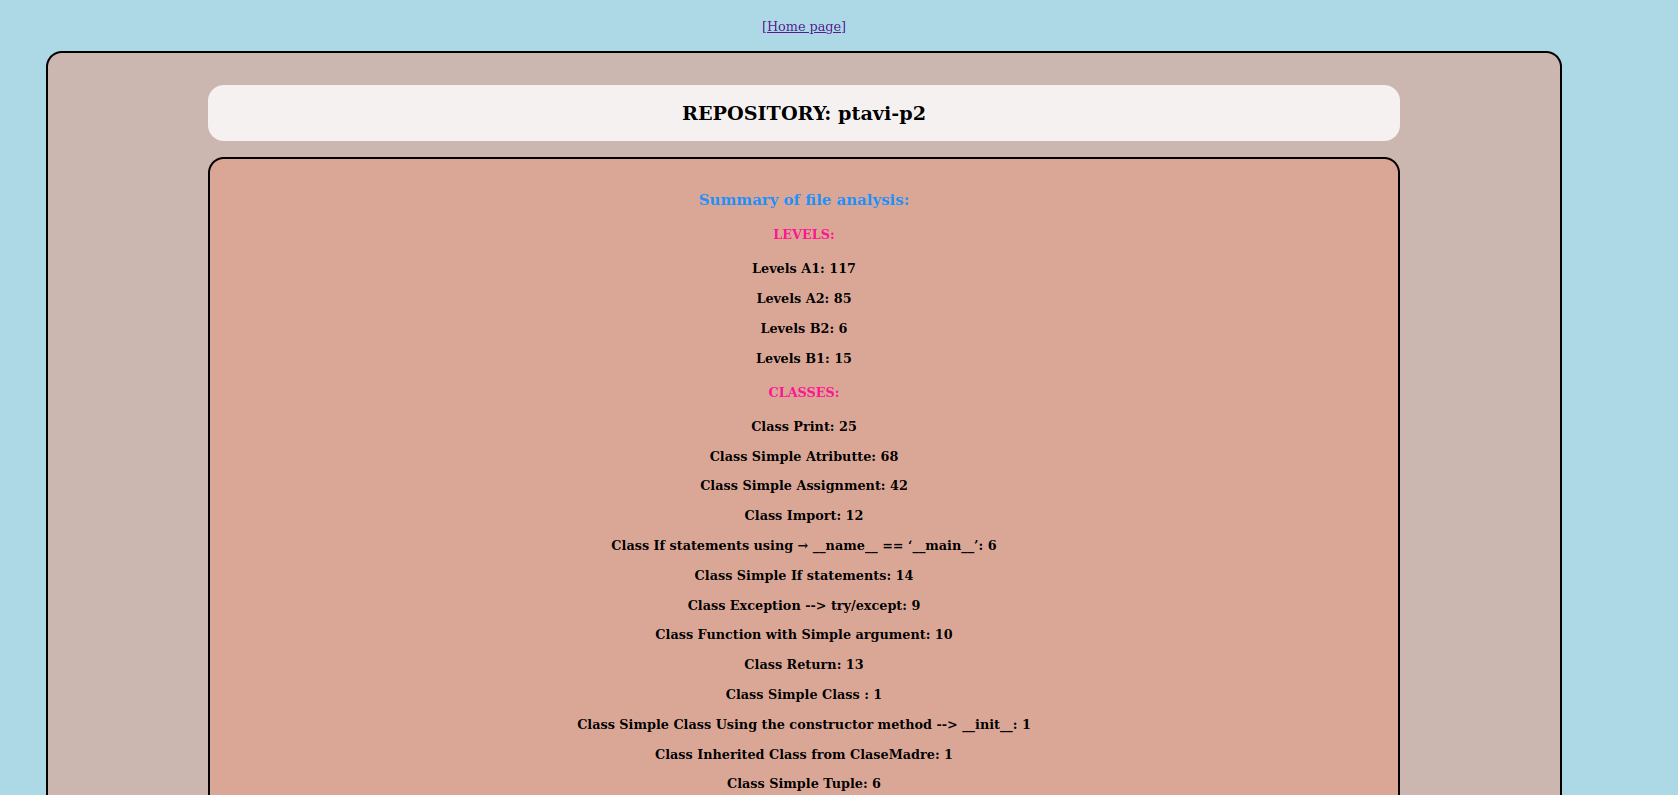
\includegraphics[width=1\textwidth]{img/ejemplousoana4.png}
  \caption{Página web del repositorio.}\label{fig:ana4}
\end{figure}

\begin{figure}
  \centering
  
\includegraphics[width=1\textwidth]{img/ejemplousoana5.png}
  \caption{Página web del fichero .py.}\label{fig:ana5}
\end{figure}

%%%%%%%%%%%%%%%%%%%%%%%%%%%%%%%%%%%%%%%%%%%%%%%%%%%%%%%%%%%%%%%%%%%%%%%%%%%%%%%%
%%%%%%%%%%%%%%%%%%%%%%%%%%%%%%%%%%%%%%%%%%%%%%%%%%%%%%%%%%%%%%%%%%%%%%%%%%%%%%%%
% DISEÑO E IMPLEMENTACIÓN %
%%%%%%%%%%%%%%%%%%%%%%%%%%%%%%%%%%%%%%%%%%%%%%%%%%%%%%%%%%%%%%%%%%%%%%%%%%%%%%%%

\cleardoublepage
\chapter{Diseño e implementación}

\section{Arquitectura general} 
\label{sec:arquitectura}

Ya se ha visto en la sección 2.2 los pasos necesarios para conseguir el objetivo principal de este proyecto. Para mostrarlo más gráficamente centrémonos en la figura~\ref{fig:arquitectura} y en la figura ~\ref{fig:_arquitectura}, la primera nos muestra como funcionaba la herramienta anteriormente y en la segunda se puede observar su funcionamiento actual.

La herramienta anteriormente, explicada con detalle en la tesis de mi compañera Ana Poveda García Herrero, contaba con un programa principal Python al cuál se le añadían parámetros por la shell indicando si se quería analizar un directorio, un repositorio o un usuario en GitHub y en el caso de que fuera un parámetro de GitHub se utilizaba su API para extraer los ficheros necesarios a analizar. En la parte izquierda de la figura ~\ref{fig:arquitectura} se destaca la clase IterTree la cual, junto con el módulo ast de árboles de sintaxis abstracta y el fichero de configuración, extraía los niveles y clases necesarias para su análisis. 

Por último, el programa principal nos devuelve los resultados por la shell además de en un formato CSV y JSON el cual se utiliza como una base de datos para poder formar la página de manera visual con HTML, JavaScript y CSS.

En el caso de la nueva herramienta mejorada, el análisis y la muestra de resultados permanece de la misma manera, el gran cambio donde se ha centrado toda la atención es en añadir dos opciones más a la lista de parámetros de objetos que se pueden analizar, en este caso, respuestas planteadas a las preguntas de Stack Overflow, página mencionada anteriormente en el capítulo 3, y código añadido a los pull request de GitHub, mencionados a su vez en el capítulo 3. Como observamos en la parte derecha de la figura ~\ref{fig:_arquitectura} vemos que si se recibe por parámetros las opciones de stack overflow o de un pull request, antes de proceder con su análisis, entra en juego un nuevo fichero Python que mediante una de las librerías de Python extrae todos los fragmentos de código de interés y posteriormente los somete a una serie de filtros y limpieza para adecuar este tipo de fragmentos al análisis que ya estaba creado con anterioridad escribiéndolos uno a uno dentro de un nuevo directorio y prescindir de aquellos que no pasen los filtros o que no sean de relevancia a la hora de analizarlos correctamente.

Finalmente, y utilizando la manera de análisis de directorios que ya había, se le devuelve al programa principal el directorio creado con todos los fragmentos de código útiles para su analisis y muestra de resultados por CSV y JSON.

\begin{figure}
  \centering
  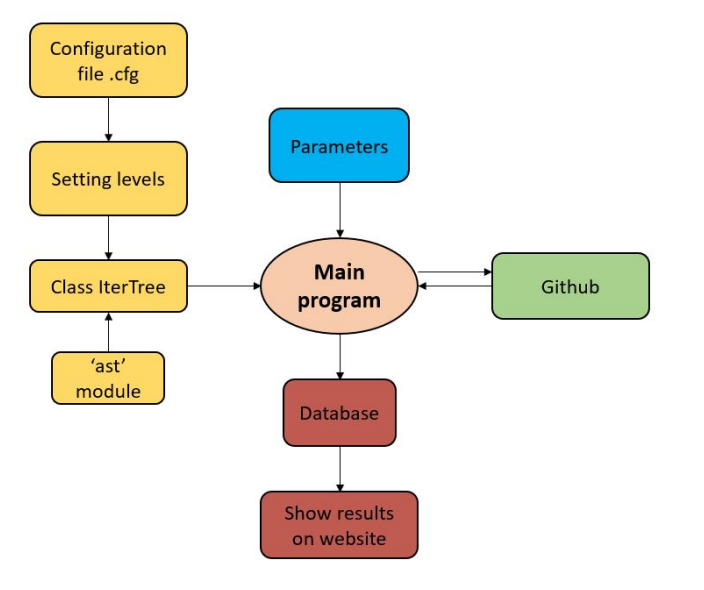
\includegraphics[width=9cm, keepaspectratio]{img/figura_funcionamiento_1.png}
  \caption{Esquema de funcionamiento principal.}\label{fig:arquitectura}
\end{figure}

\begin{figure}
    \centering
    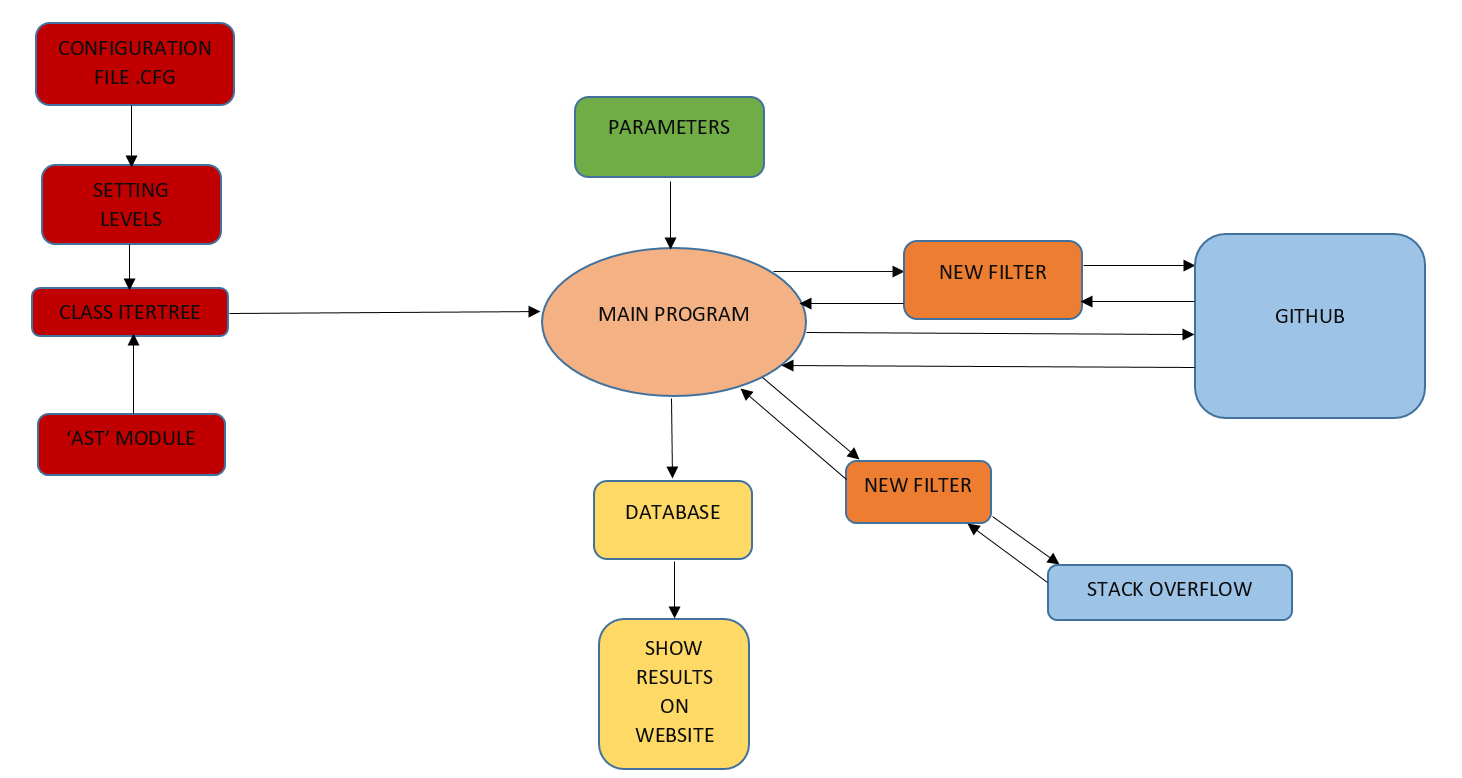
\includegraphics[bb=0 0 800 600, width=12cm, keepaspectratio]{img/figura_funcionamiento_2}
    \caption{Esquema de funcionamiento mejorado.}\label{fig:_arquitectura}
\end{figure}

\section{Obtención de ficheros en las diferentes opciones} 
\label{sec:Obtención de ficheros en las diferentes opciones}

En este punto y una vez ejecutado el fichero de configuración (explicado en el capitulo 5) podemos enviar al programa principal distintas parejas de opción y valor según lo que queramos analizar.

las distintas opciones son:

\begin{itemize}
	\item \textbf{Directory:} En este caso el valor que debe ir con esta opción tiene que ser una ruta a una carpeta en específico. Ya que, como la propia definición de directorio especifica, debe ser una carpeta contenedora de archivos y otros subdirectorios. Un ejemplo de esto podría ser:
	\begin{verbatim}
	Users\jjime\Escritorio\tfg
	\end{verbatim}
	\item \textbf{repo-url:} En este caso el valor que lo acompaña debe ser una URL asociada a un repositorio alojado en GitHub. Para conseguir esto debemos ir a cualquier repositorio que queramos analizar en GitHub, pulsar en el botón `clone' y copiar la URL de https. Un ejemplo de esto podría ser:
	\begin{verbatim}
	https://github.com/jjramiro/pycefr.git
	\end{verbatim}
	\item \textbf{user:} En este caso el valor que acompaña a esta opción debe ser un usuario de GitHub cualquiera. Con esto analizara todos los repositorios de ese usuario, un ejemplo podría ser:
	\begin{verbatim}
	jjramiro
	\end{verbatim}
	\item \textbf{stack:} Este es uno de los nuevos casos añadidos. El valor que debe de acompañar a esta opción es una URL de la web de Stack Overflow mencionada en capítulos anteriores. Para conseguir un valor valido debemos irnos a web de Stack Overflow y pulsar en el apartado `questions', una vez ahí aplicaremos el filtro de Python 3.X y entrar en la pregunta que más nos interese y copiar la URL completa. Un ejemplo de esto podría ser:
	\begin{verbatim}
	https://stackoverflow.com/questions/606191/
	convert-bytes-to-a-string
	\end{verbatim}
	\item \textbf{pull:} Este el segundo de los nuevos  casos añadidos. El valor que acompaña a este caso es la URL en github de un pull-request mencionado en el capítulo 3. Para conseguir un valor correcto debemos irnos a GitHub y buscar un proyecto escrito en su mayoría en Python y entrar en él, una vez ahí pulsamos en el apartado de `pull requests', pulsamos en cualquiera de los que nos aparecen y copiamos la URL completa. Un ejemplo de esto podría ser:
	\begin{verbatim}
	https://github.com/TheAlgorithms/Python/pull/6209
	\end{verbatim}
\end{itemize}

En el primer caso comienza el análisis del directorio sin problemas indicando el proceso por la shell, en el segundo y tercer caso son algo más complejos ya que se hace uso de la API de GitHub para hacer peticiones GET y así clonar el repositorio únicamente si supera la mitad de código en Python. Estas tres opciones ya estaban anteriormente explicadas y hechas en la tesis de mi compañera Ana así que en los siguientes puntos nos vamos a centrar en profundidad en la obtención de los ficheros a analizar en las últimas dos opciones.

\section{Lectura y extracción de los fragmentos de interés} 
\label{sec:Obtención de ficheros en las diferentes opciones}

En este punto nos vamos a centrar en como se extraen los fragmentos de código útiles para su análisis de las últimas dos opciones comentadas anteriormente.

Ejecutando o bien la opción de `stack' o bien la opción de `pull' con una URL correcta nos llevará al nuevo fichero Python de análisis añadido. las formas de extracción dependiendo de la opción serán las siguientes.

\subsection{Lectura y extracción de Stack Overflow}

En el caso de Stack Overflow comenzamos haciendo una pequeña comprobación de que la URL es correcta, comprobando si la URL contiene el nombre de la web, el apartado de preguntas, denominado `questions', y el protocolo https.

Si la URL no tiene ningún fallo podemos pasar a la lectura de la web. Para ello utilizamos la librería de 
Python `urllib'~\cite{website:Urllib} que nos permite obtener el HTML completo de la página en cuestión, además, como esta organizado por etiquetas podemos aislar cada uno de los fragmentos de código, en este caso de las respuestas, que sean útiles para analizar.

Una vez realizado este aislamiento de todos los fragmentos de código mediante las etiquetas de HTML nos queda una lista con todos los fragementos o `snippets' de las respuestas. Con esto podemos proceder a su limpieza y análisis.

\subsection{Lectura y extracción de Pull requests}

Igual que en el caso anterior lo primero que debemos hacer es una pequeña comprobación de que la URL es correcta, comprobando que la URL contenga el nombre de la web de GitHub y que el protocolo sea https.

Teniendo la URL correcta podemos pasar a la lectuar de la web igual que hacimaos en la parte anterior pero creando una nueva web de mayor interés mediante la web de github proporcianada, por lo tanto, si la web proporcionada es por ejemplo:
\begin{verbatim}
https://github.com/TheAlgorithms/Python/pull/6209
\end{verbatim}

La nueva web creada para la extracción de ficheros sería tal que:

\begin{verbatim}
https://patch-diff.githubusercontent.com/raw/
TheAlgorithms/Python/pull/6209.diff
\end{verbatim} 

Esta nueva web nos da acceso a los archivos diff\footnote{https://docs.kde.org/stable5/es/kompare/kompare/working-with-diff-files.html} dentro del pull request seleccionado, estos archivos son los fragmentos de código que han sido añadidos, eliminados o cambiados comparándolos con la rama principal del proyecto, así nos es mucho más sencillo aislar los fragmentos de interés para el análisis.

Teniendo esta web la manera de proceder a su lectura y extracción es muy sencilla, extraemos el HTML de la web con la misma librería mencionada anteriormente y después solo nos queda eliminar las cabeceras de cada uno de los fragmentos.

Con esto conseguimos una lista de los fragmentos que nos interesan preparados para su limpieza y análisis.

\section{limpieza y análisis de los fragmentos obtenidos} 
\label{sec:limpieza y análisis de los fragmentos obtenidos}

En este punto de la extracción tenemos una lista completa con todos los fragmentos de código que pueden ser interesantes para el análisis, pero aun no están perfilados por completo ya que tenemos estos fragmentos en `crudo'.

Por lo tanto para que el análisis sea lo más correcto posible hay que cambiar algunas partes dentro de estos fragmentos como símbolos incompatibles, por ejemplo el inicio de la shell de Python\footnote{https://pythondiario.com/2013/04/el-interprete-de-python-o-shell.html}, partes aún en html o caracteres especiales\footnote{https://ascii.cl/es/codigos-html.htm}.

Para solucionar este problema se han añadido varios filtros por los que tiene que pasar el fragmento para permitirle ser analizado correctamente.

\subsection{limpieza de los fragmentos Stack Overflow}

Como se comentaba en el capítulo 4.3.1 ya tenemos los fragmentos necesarios y podemos comenzar a su limpieza mediante los filtros, para esta tarea y sabiendo que en una web como stack overflow cada usuario puede escribir los fragmentos de código de la manera que quiera e incluso poner fragmentos incompletos o en otro tipo de lenguajes que no sean Python3 como en texto plano, se han ideado los filtros pensando en las complicaciones más comunes y queriendo abarcar los problemas con mayor probabilidad.

los distintos filtros que se han ideado son:

\begin{enumerate}
	\item Para el primer filtro se hace uso de una de las librerías de Python llamada html~\cite{website:libreriahtml}. Con esta librería transformamos todos los caracteres especiales en formato html a su formato en ascii\footnote{https://elcodigoascii.com.ar/} que es el que nos interesa.
	\item El siguiente filtro que entra en acción es para intentar eliminar todos aquellos fragmentos que se basen en un error mostrado por la línea de comandos y los que se basen en comandos en sí, si aparecen una de estas dos cosas ignoramos el fragmento ya que no tendrá nada de utilidad en el análisis. además en este mismo momento también se ignoran todos aquellos fragmentos que sean solo una palabra ya que no tendría sentido el analizarla.
\end{enumerate}

Todos aquellos fragmentos que hayan llegado hasta aquí merecen ser guardados ya que podrían tener utilidad, pero aun quedan algunos filtros de limpieza que aplicar. Antes de seguir con la limpieza se crean archivos .py para guardar, con un nombre distintivo, todas las respuestas que podrían ser útiles. A cada fragmento se le nombra siguiendo el siguiente patrón:

\begin{verbatim}
answer_ + número de respuesta + _file_ + número del fragmento + .py
\end{verbatim}

Con los fragmentos guardados podemos proseguir con los siguientes filtros:

\begin{enumerate}
	\item Para el siguiente filtro pasamos el fragmento por una función que se encarga de dividir este fragmento por líneas para eliminar todos los símbolos y caracteres que tengan que ver con la estructura de la shell de Python para así obtener únicamente el código útil.
	\item El siguiente filtro se encarga de los saltos de línea, estos se indican con las barras invertidas y la letra `n', pero al extraer el código la barra invertida se duplica por lo tanto debemos eliminar esa barra extra para no causar ningún error en el análisis.
	\item Para terminar aplicamos el último filtro que consta de una función que se encarga de eliminar todos aquellos fragmentos que solo posean una línea de código ya que aunque podrían llegar a ser correctos al pasar por el análisis no influye en el nivel CEFRL de la respuesta por lo tanto solo aplican un mayor tiempo de ejecución y no son eficientes.
\end{enumerate}

Una vez hecho esto dentro del directorio solo quedan las respuestas útiles y se puede proceder con su análisis.

\subsection{limpieza de los fragmentos Pull-Requests}

Igual que en el caso de Stack Overflow y como se comentaba en el capítulo 4.3.2, ya tenemos una lista con todos los fragmentos listos para su limpieza y análisis, pero al contrario que en el punto anterior en esta parte solo nos tenemos que preocupar de algunos caracteres de control (comienzan con la barra invertida) o algunos mensajes de aviso que se `cuelan' en el fragmento seleccionado.

Para abordar los problemas más comunes ideamos los siguientes filtros:

\begin{enumerate}
	\item El primer filtro nos permite ignorar todos los fragmentos de menos de 50 caracteres que, aunque puedan tener un análisis correcto, son demasiado pequeños y no interesa su análisis ya que no variará mucho el resultado y solo molestarían a la ejecución del análisis.
\end{enumerate}

Los fragmentos que pasen de este primer filtro merecen ser guardados ya que podrían tener utilidad, pero igual que antes aun quedan algunos filtros de limpieza que aplicar. Antes de seguir con la limpieza se crean archivos .py al igual que en el punto anterior para guardar, con un nombre distintivo, todos los fragmentos que nos sean de utilidad. A cada fragmento se le nombra siguiendo el siguiente patrón:
 
\begin{verbatim}
pull_ + número del fragmento + .py
\end{verbatim}

Una vez guardados podemos proseguir con los filtros de limpieza que nos quedan:

\begin{enumerate}
	\item Para el siguiente filtro debemos eliminar algunos caracteres que aparecen en todos los pull requests cuando hay cambios o cuando se añaden y eliminan líneas de código. Estos caracteres suelen ser el signo + y el signo -, así que para eliminarlos del comienzo de todas las líneas pasamos el fragmento por una función que elimina el primer carácter de todas las líneas dejando el código mucho más limpio.
	\item En el siguiente filtro de limpieza nos encargamos de eliminar tanto los simbolos de inicio de la shell de Python, al igual que en el apartado anterior, como algunos caracteres invisibles formados por la barra invertida y una letra. Con los caracteres invisibles llamados caracteres de controlo solo nos encargamos de eliminar una de las barras invertidas por estar duplicada. Estos caracteres son:
	\begin{itemize}
		\item El primero de ellos es la barra invertida seguida de una `n' que representa el salto de línea.
		\item el segundo es la misma barra invertida seguida de una `t' que equivale a el tabulador del teclado.
		\item el tercero equivale a esta misma barra invertida seguida de una `r' que equivale al retorno de carro (tecla enter).
	\end{itemize}
	\item En el último de estos filtros solamente eliminamos un mensaje de aviso que aparece al final de los pull-requests precedido de una doble barra invertida que se produce cuando el fragmento no tiene una línea en blanco al final del mismo.
\end{enumerate}

Una vez habiendo terminado con los filtros ya solo quedan en el directorio los fragmentos listos para su análisis.

\subsection{Análisis y resultados}

Por último y acabando con este proceso, ya tenemos todos los fragmentos reunidos en un directorio y separados en ficheros .py listos para su análisis. Por ello, le devolvemos la ruta donde se encuentran estos fragmentos al programa principal, y aprovechando la opción de análisis de directorios, procedemos a el análisis de todos los fragmentos.

Aun habiendo pasado por tantos filtros, y sabiendo que Stack Overflow y la parte de Pull-Requests de GitHub son tan extensas, aun pueden ocurrir errores durante el análisis por pequeños fallo que no se han tomado en cuenta por la dificultad que supone solucionarlos y porque a grandes rasgos no son significativos.

Después del análisis completo se generan tanto un pequeño resumen mostrado por la línea de comandos, como una `base de datos' en JSON, y otra en CSV que nos serán útiles si queremos mostrar los resultados finales de forma mas gráfica y específica mediante la creación de una página web ya disponible en la versión anterior de esta herramienta y creada por mi compañera Ana. 

A continuación veremos en las figuras \ref{fig:uso1}, \ref{fig:uso2}, \ref{fig:uso3}, \ref{fig:uso4}, \ref{fig:uso5}, \ref{fig:uso6}, \ref{fig:uso7}, \ref{fig:uso8}, \ref{fig:uso9}, \ref{fig:uso10}, un ejemplo de uso del apartado de Stack Overflo y del apartado de Pull Request.

\begin{figure}
  \centering
  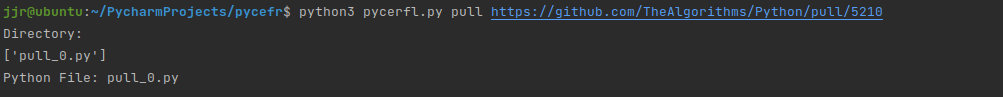
\includegraphics[width=1\textwidth]{img/uso1.png}
  \caption{Ejemplo de ejecución Pull Request.}\label{fig:uso1}
\end{figure}

\begin{figure}
  \centering
  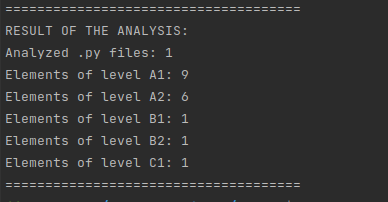
\includegraphics[width=9cm, keepaspectratio]{img/uso2.png}
  \caption{Resultado de análisis Pull Request.}\label{fig:uso2}
\end{figure}

\begin{figure}
  \centering
  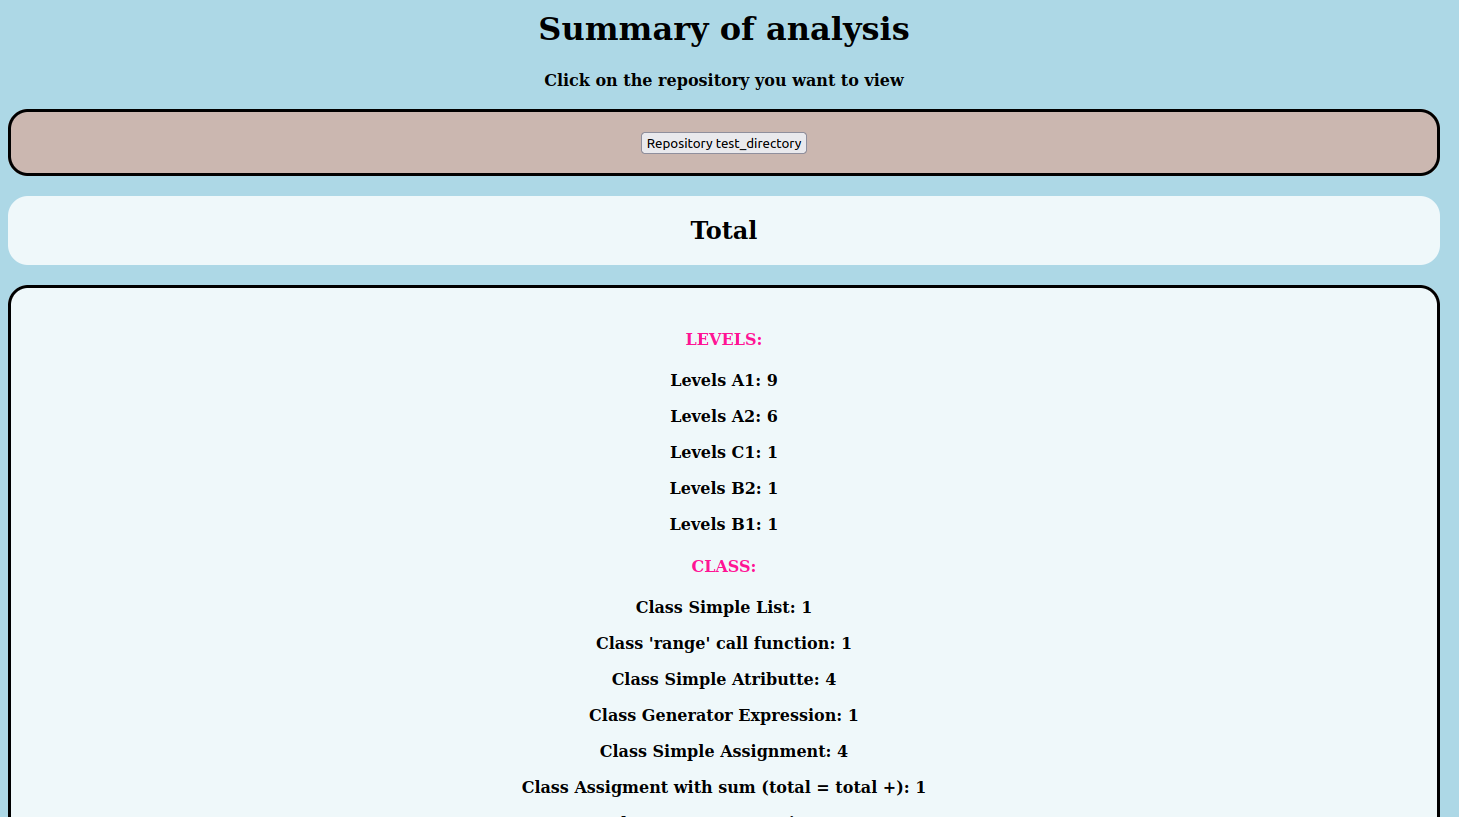
\includegraphics[width=1\textwidth]{img/uso3.png}
  \caption{Página web principal.}\label{fig:uso3}
\end{figure}

\begin{figure}
  \centering
  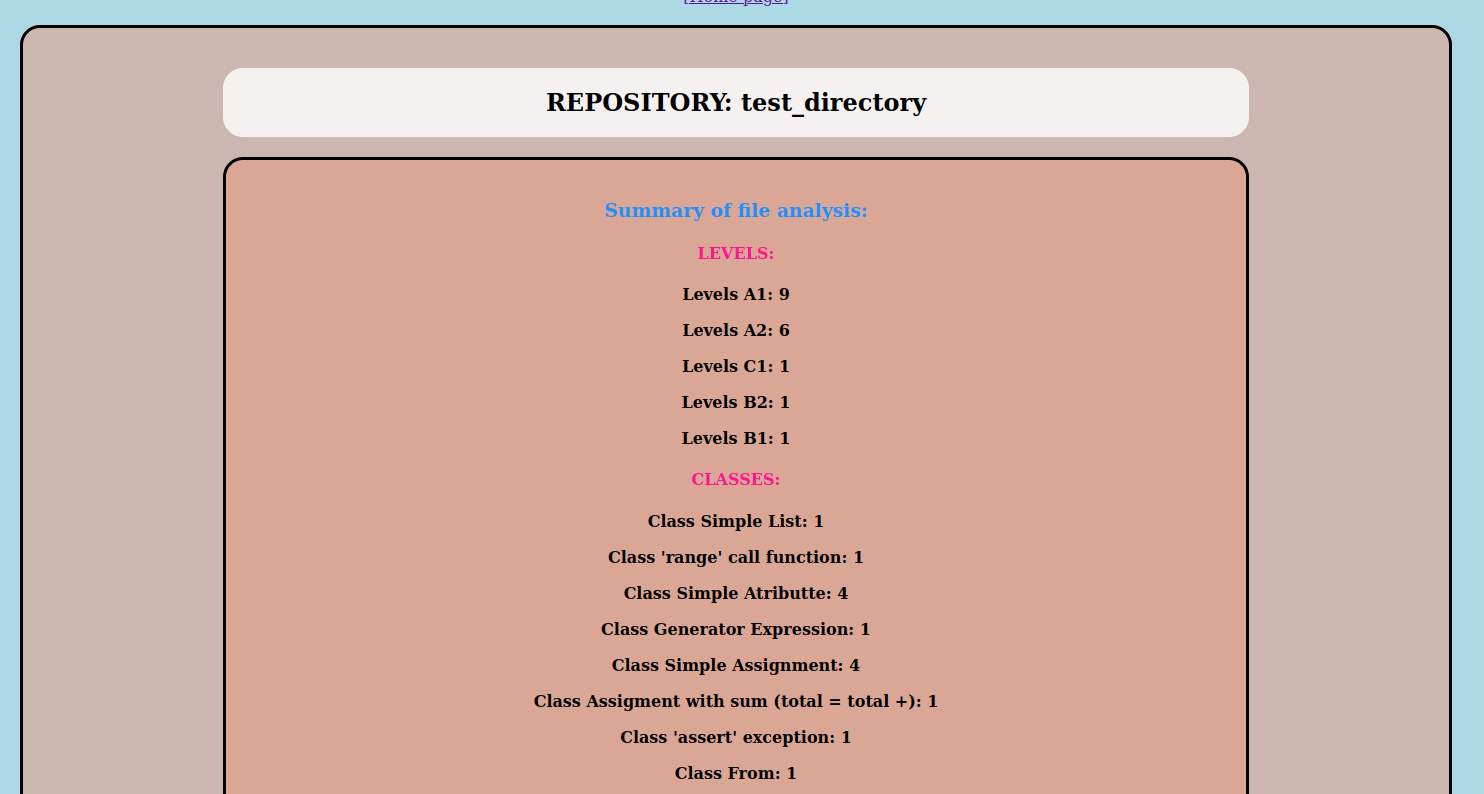
\includegraphics[width=1\textwidth]{img/uso4.png}
  \caption{Página web del Pull Request.}\label{fig:uso4}
\end{figure}

\begin{figure}
  \centering
  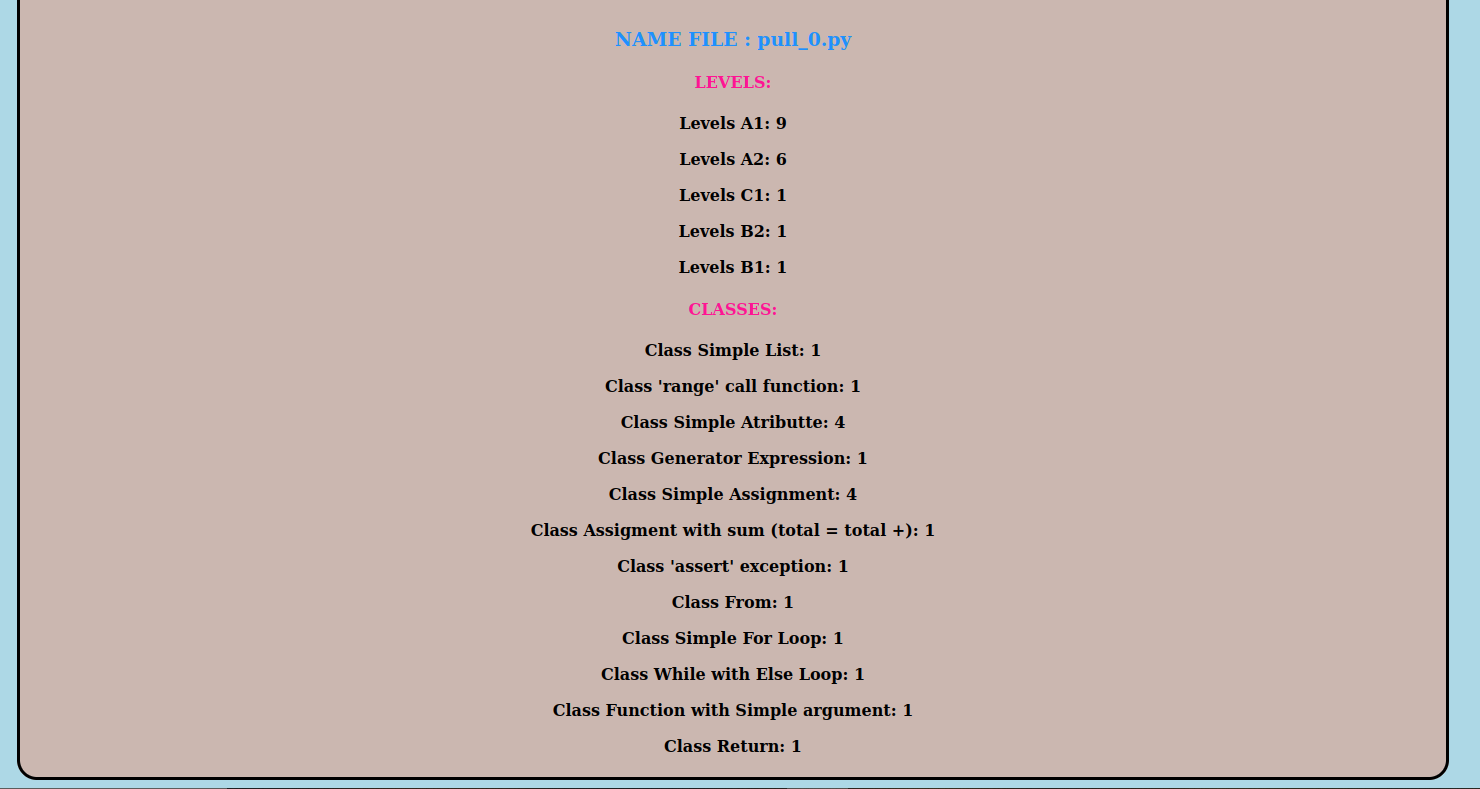
\includegraphics[width=1\textwidth]{img/uso5.png}
  \caption{Página web del fichero .py.}\label{fig:uso5}
\end{figure}

\begin{figure}
  \centering
  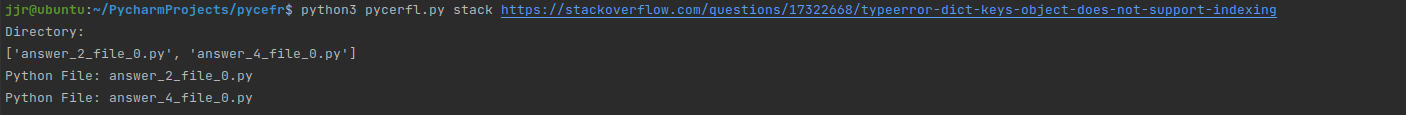
\includegraphics[width=1\textwidth]{img/uso6.png}
  \caption{Ejemplo de ejecución Stack Overflow.}\label{fig:uso6}
\end{figure}

\begin{figure}
  \centering
  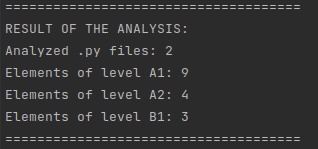
\includegraphics[width=9cm, keepaspectratio]{img/uso7.png}
  \caption{Resultado de análisis Stack Overflow.}\label{fig:uso7}
\end{figure}

\begin{figure}
  \centering
  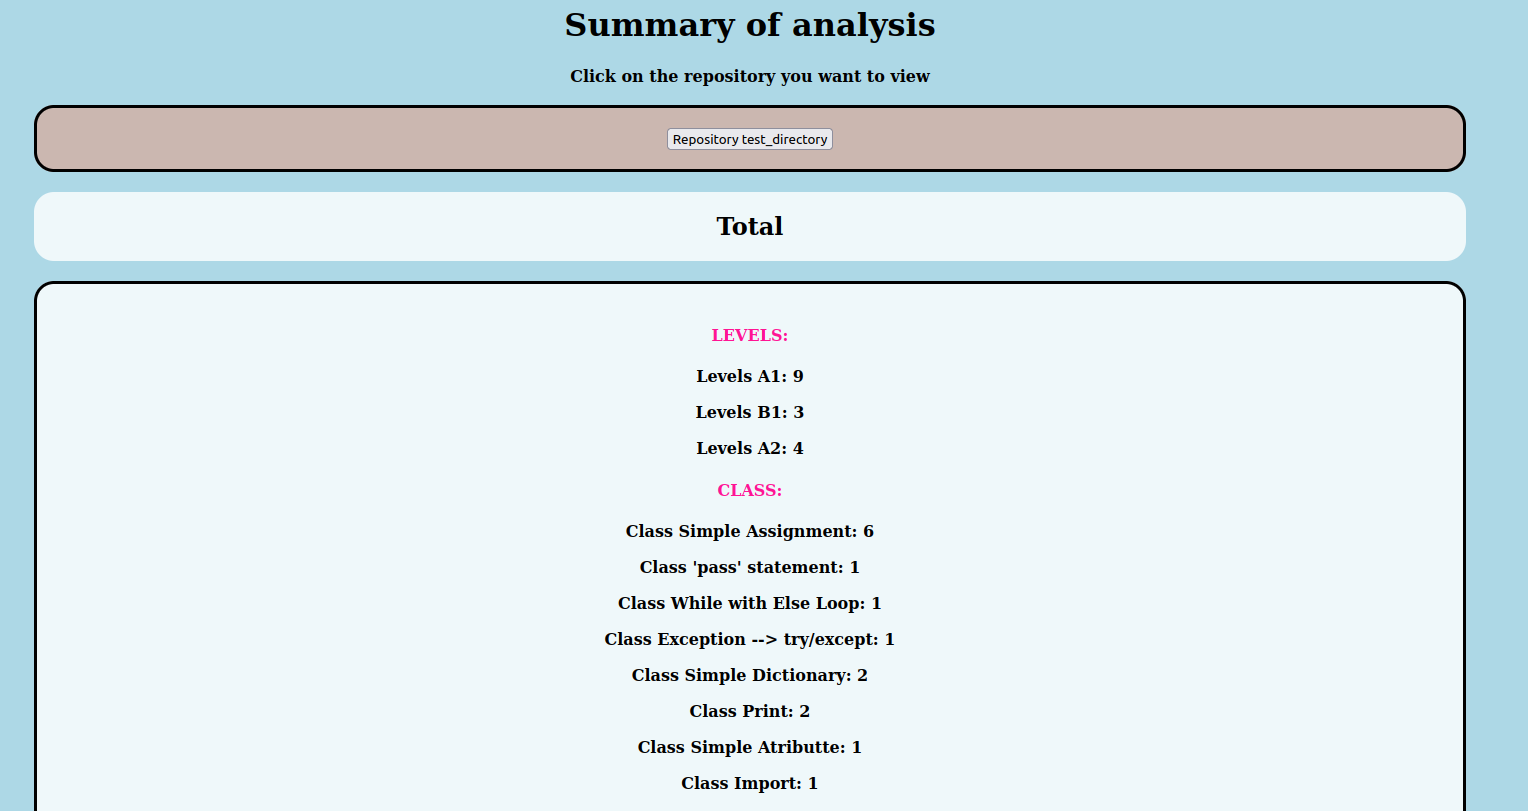
\includegraphics[width=1\textwidth]{img/uso8.png}
  \caption{Página web principal.}\label{fig:uso8}
\end{figure}

\begin{figure}
  \centering
  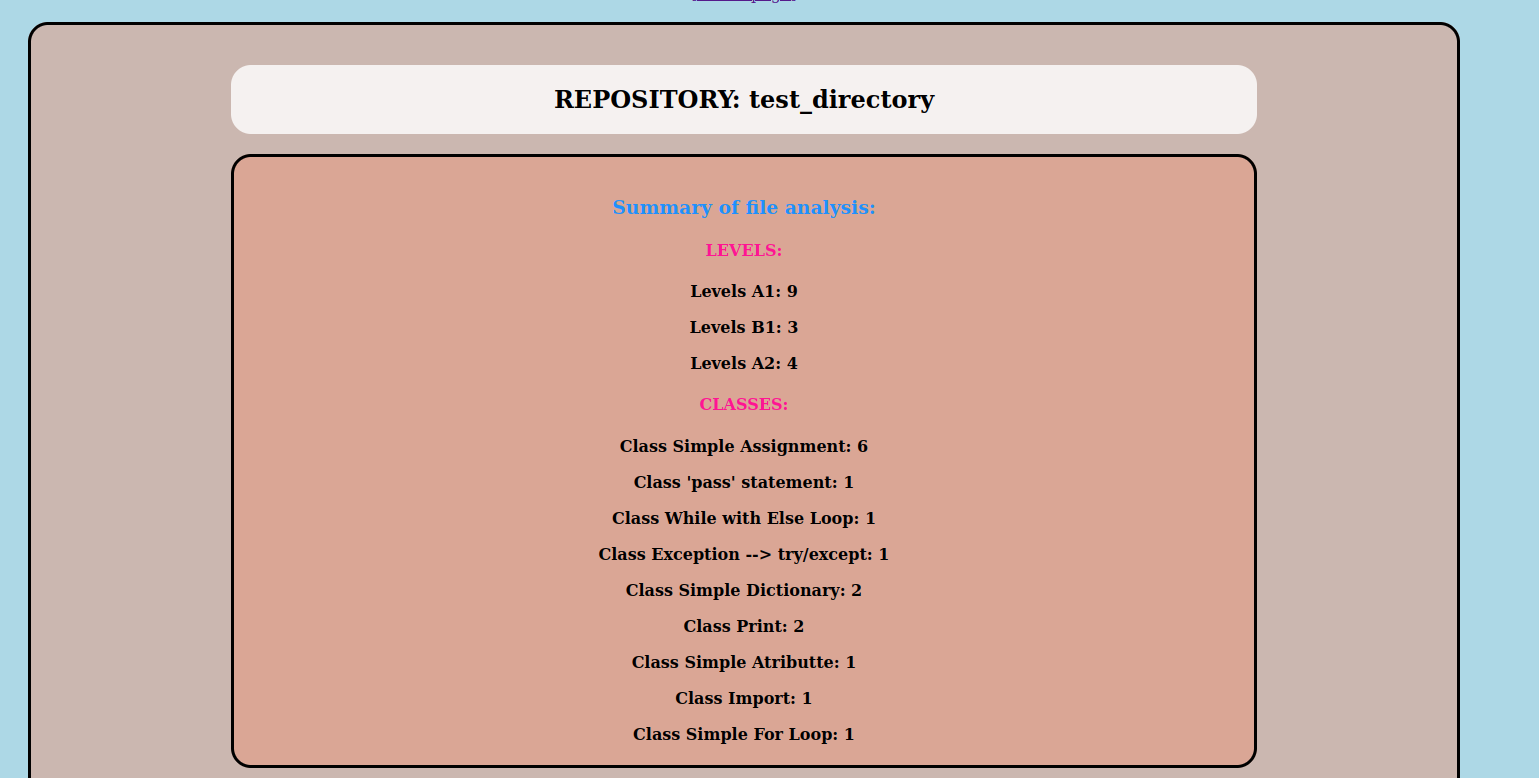
\includegraphics[width=1\textwidth]{img/uso9.png}
  \caption{Página web de resultado Stack Overflow.}\label{fig:uso9}
\end{figure}

\begin{figure}
  \centering
  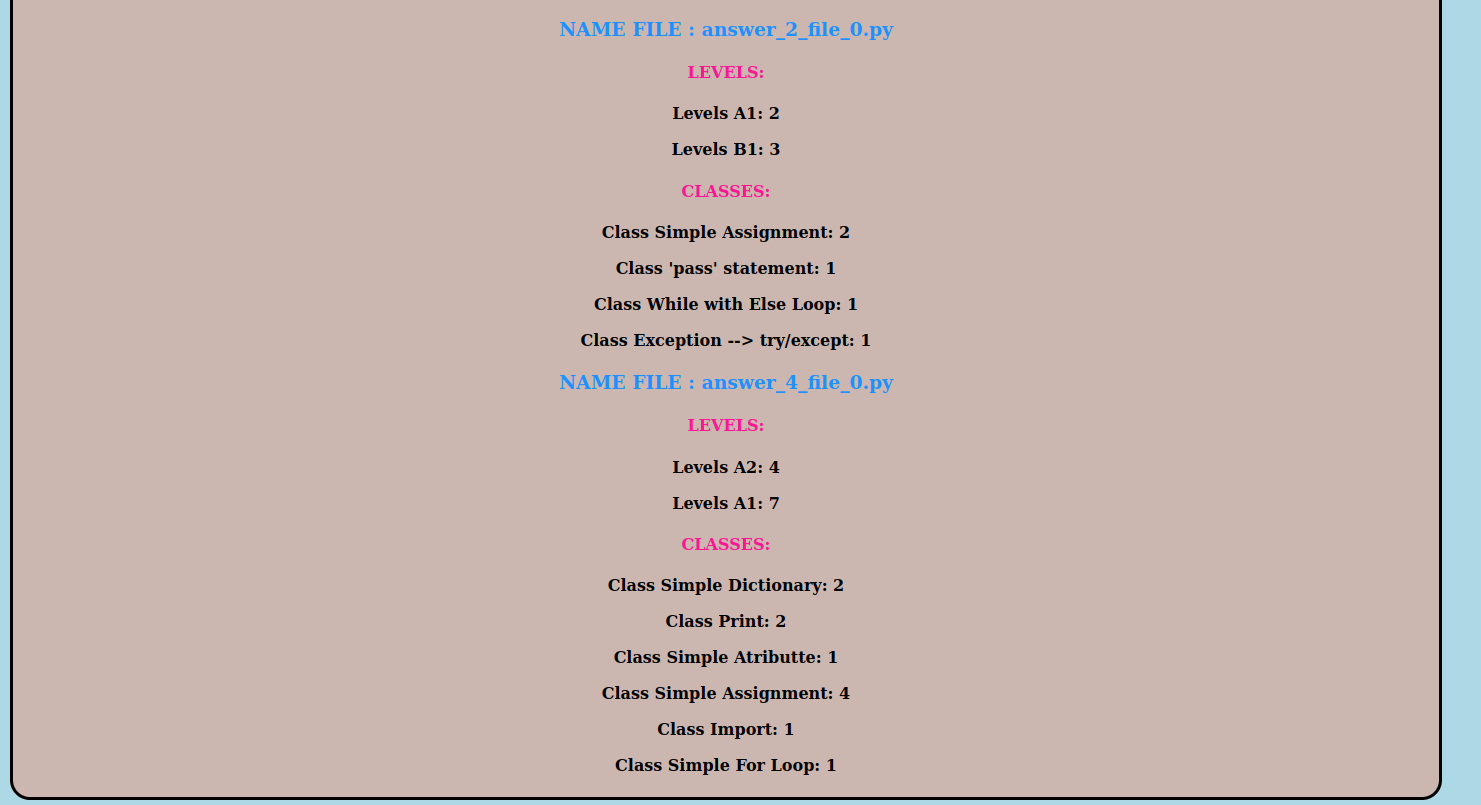
\includegraphics[width=1\textwidth]{img/uso10.png}
  \caption{Página web del fichero .py.}\label{fig:uso10}
\end{figure}



%%%%%%%%%%%%%%%%%%%%%%%%%%%%%%%%%%%%%%%%%%%%%%%%%%%%%%%%%%%%%%%%%%%%%%%%%%%%%%%%
%%%%%%%%%%%%%%%%%%%%%%%%%%%%%%%%%%%%%%%%%%%%%%%%%%%%%%%%%%%%%%%%%%%%%%%%%%%%%%%%
% RESULTADOS %
%%%%%%%%%%%%%%%%%%%%%%%%%%%%%%%%%%%%%%%%%%%%%%%%%%%%%%%%%%%%%%%%%%%%%%%%%%%%%%%%

\cleardoublepage
\chapter{Manual de Usuario}

En este capitulo abordaremos una correcta utilización y configuración, desde el inicio hasta los resultados, de la herramienta desarrollada mediante un manual de usuario centrándose en las dos nuevas opciones añadidas.

Lo primero que debemos hacer es obtener la herramienta de forma local desde GitHub. Para ello primero debemos hacer un `fork'\footnote{https://desarrolloweb.com/articulos/fork-git}, basicamente copiar el repositorio de la rama principal a nuestro perfil de usuario. Después, se debe clonar este repositorio de forma local para poder utilizarlo y editarlo\footnote{https://docs.github.com/es/repositories/creating-and-managing-repositories/cloning-a-repository}.

Una vez que lo tenemos en local empezaremos con la creación de un fichero de configuración. Este fichero sirve para determinar y fijar los distintos tipos de niveles CEFRL en Python. en este caso y aunque se pueda personalizar completamente vamos a utilizar el que esta hecho por defecto.

Para ello ejecutaremos en nuestra shell dentro del directorio local de nuestra herramienta el siguiente comando:

\begin{verbatim}
	python3 dict.py
\end{verbatim}

Ejecutando este comando ya tenemos el fichero de configuración listo y ahora podemos pasar a ejecutar el comando para el análisis de cada una de las opciones disponibles.

\begin{itemize}
	\item Para el análisis de un repositorio Github:
	\begin{verbatim}
	python3 pycerfl.py repo <name_urlclone>
	\end{verbatim}
	\item Para el análisis de un usuario Github:
	\begin{verbatim}
	python3 pycerfl.py user <name_user>
	\end{verbatim}
	\item Para el análisis de un directorio local:
	\begin{verbatim}
	python3 pycerfl.py directory <name_path>
	\end{verbatim}
\end{itemize}

Pero nos centraremos como he mencionado anteriormente en el análisis de Stack Overflow y en el análisis de los Pull-Requests.

\section{Manual de análisis Stack Overflow}

Para comenzar con este análisis entraremos en la página web de Stack Overflow:

\begin{verbatim}
https://stackoverflow.com/
\end{verbatim}

Una vez dentro pulsaremos en las tres líneas de la parte superior izquierda que vemos en la figura \ref{figura:stack1} y pulsaremos en el apartado `questions'.

\begin{figure}
    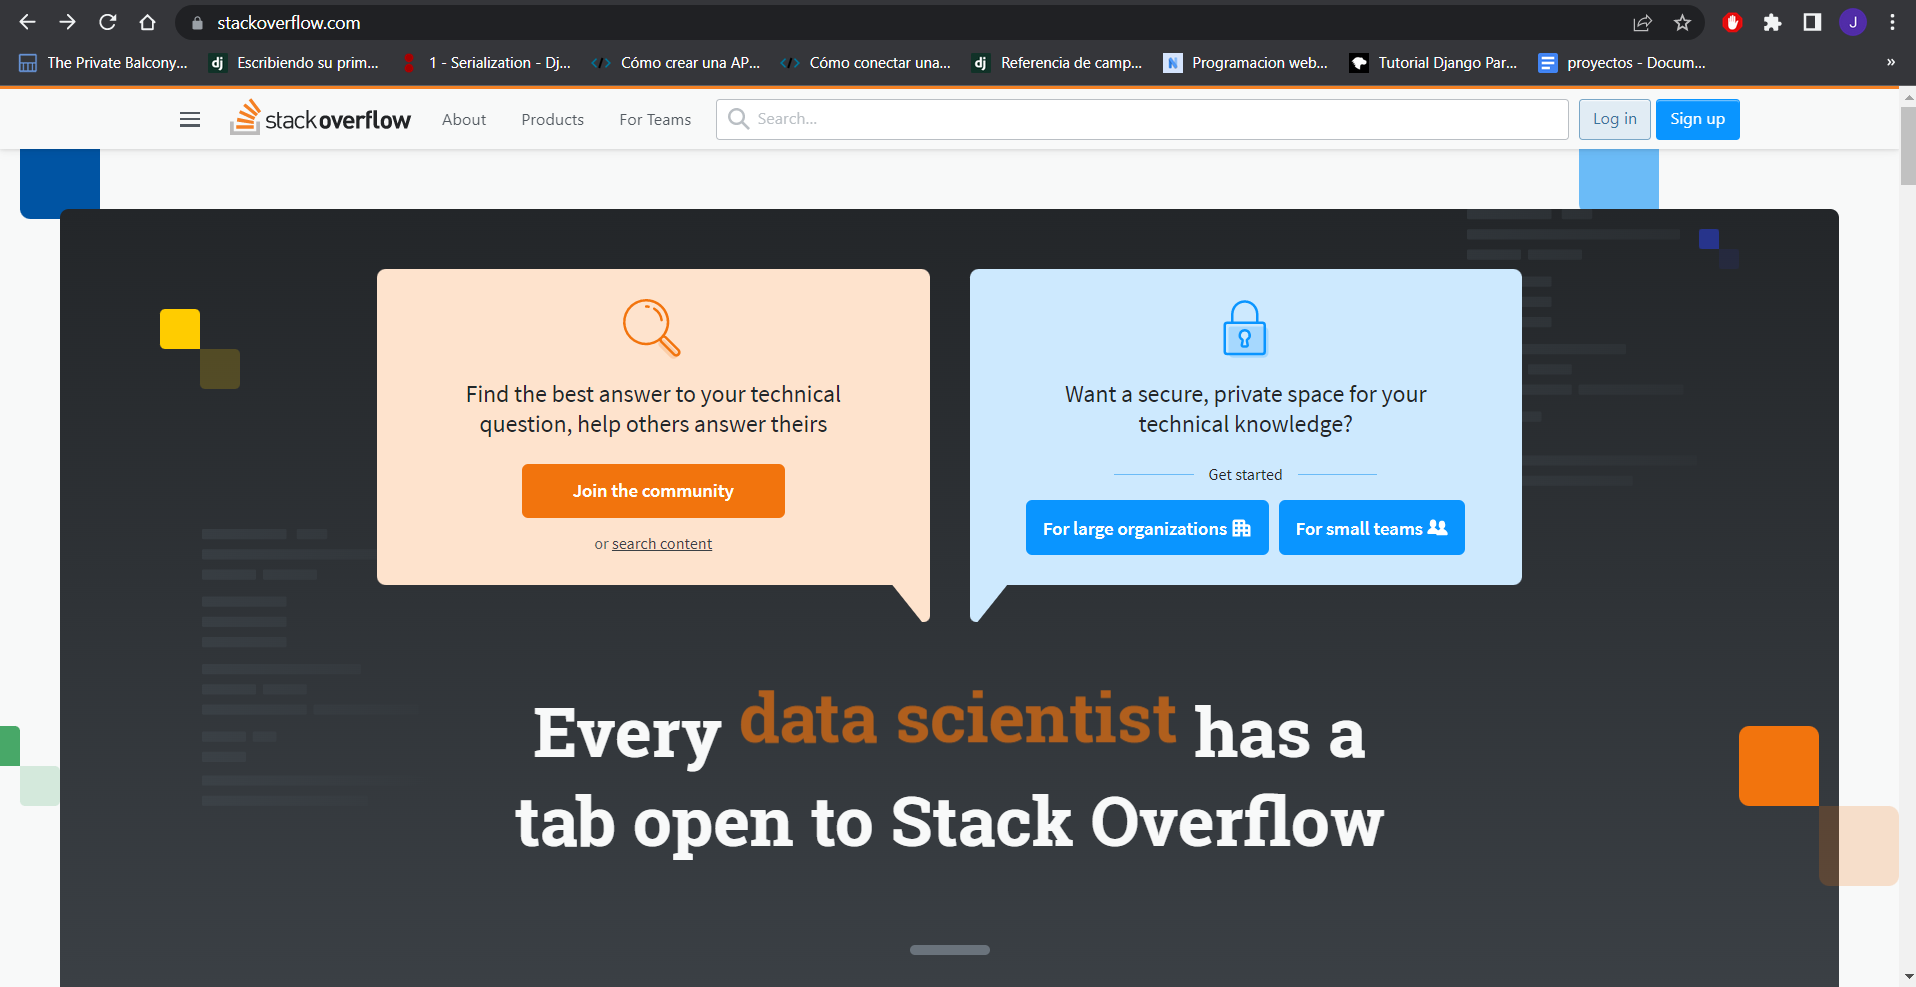
\includegraphics[bb=0 0 800 600, width=12cm, keepaspectratio]{img/stack1}
    \caption{Pagina principal de Stack Overflow}
    \label{figura:stack1}
 \end{figure}
 
En el apartado de las preguntas veremos algo como lo que aparece en la figura \ref{figura:stack2}. En esta parte pulsaremos en el botón `filter' y buscaremos, dentro del apartado de `the following tags', la etiqueta clave `python3'. Una vez hecho esto pulsamos en `apply filter'.

\begin{figure}
    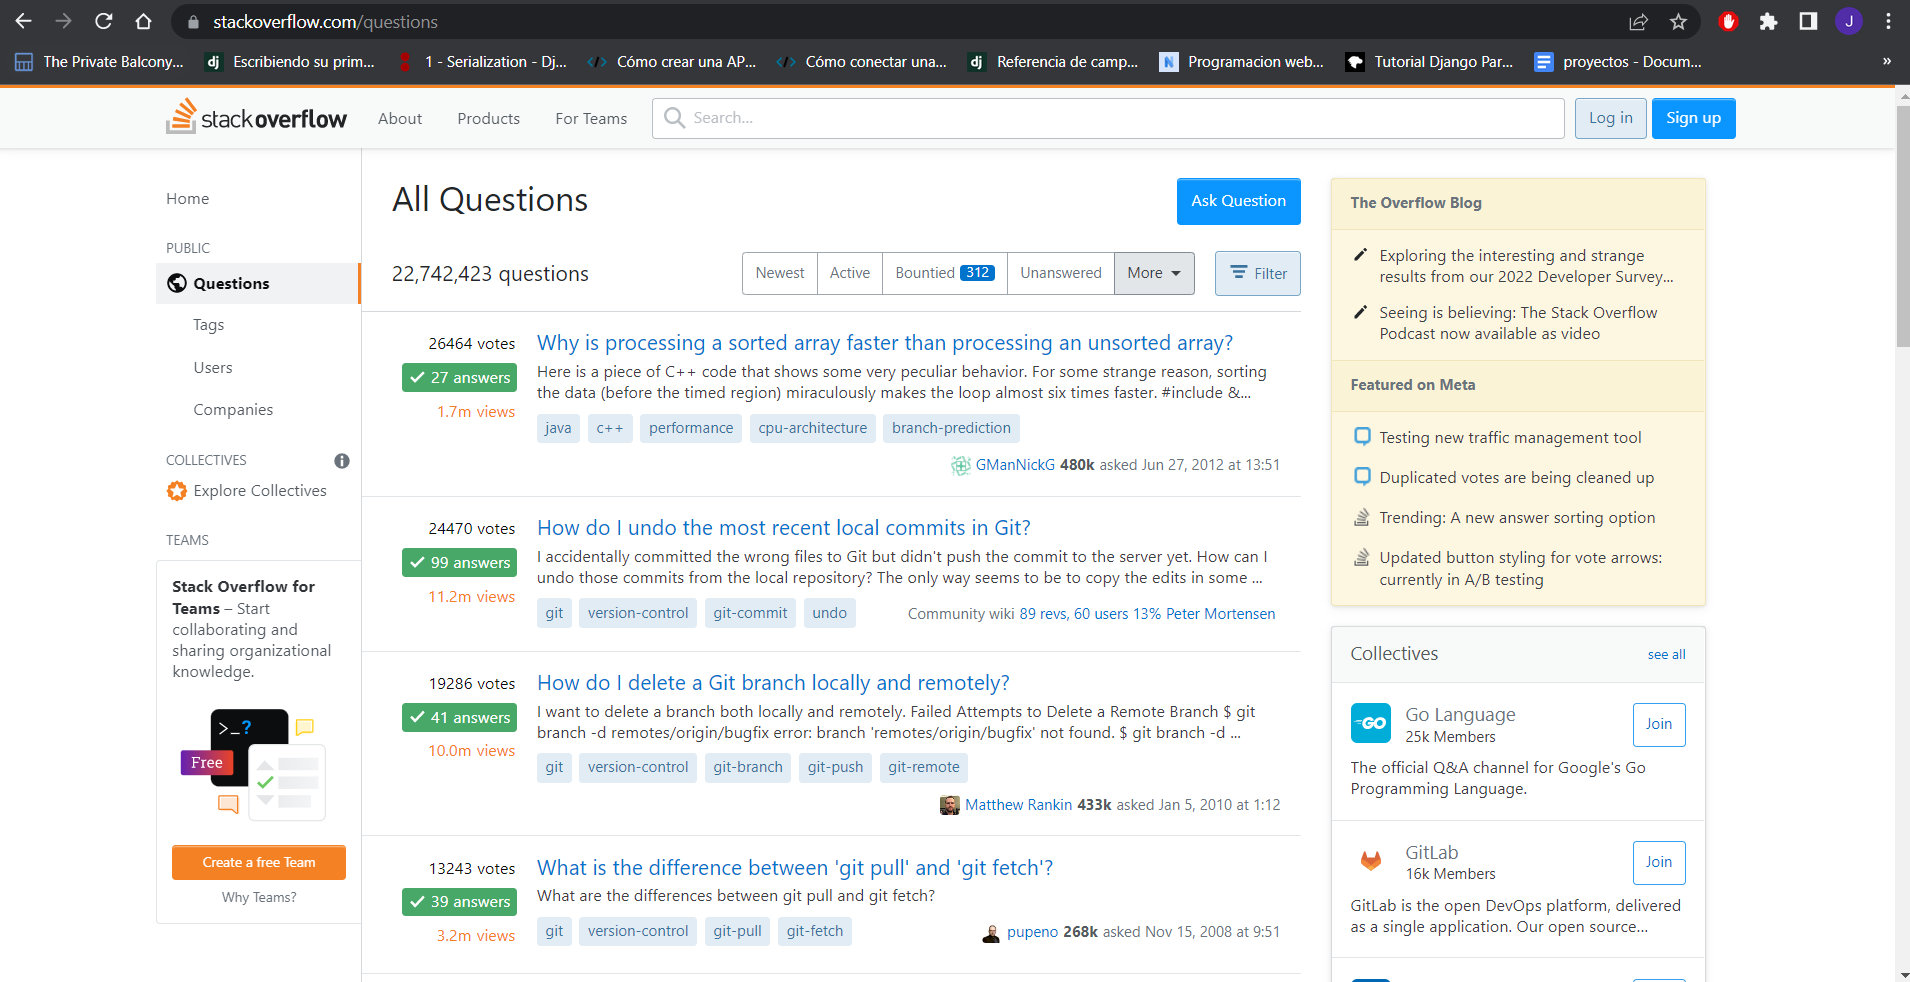
\includegraphics[bb=0 0 800 600, width=12cm, keepaspectratio]{img/stack2}
    \caption{Pagina de preguntas de Stack Overflow}
    \label{figura:stack2}
 \end{figure}
 
Con esto nos aseguraremos de que todas las preguntas que aparecen son sobre Python y podremos analizarlas. Ahora podemos pulsar en cualquiera de las preguntas y nos aparecerá algo como la figura \ref{figura:stack3}. 


\begin{figure}
    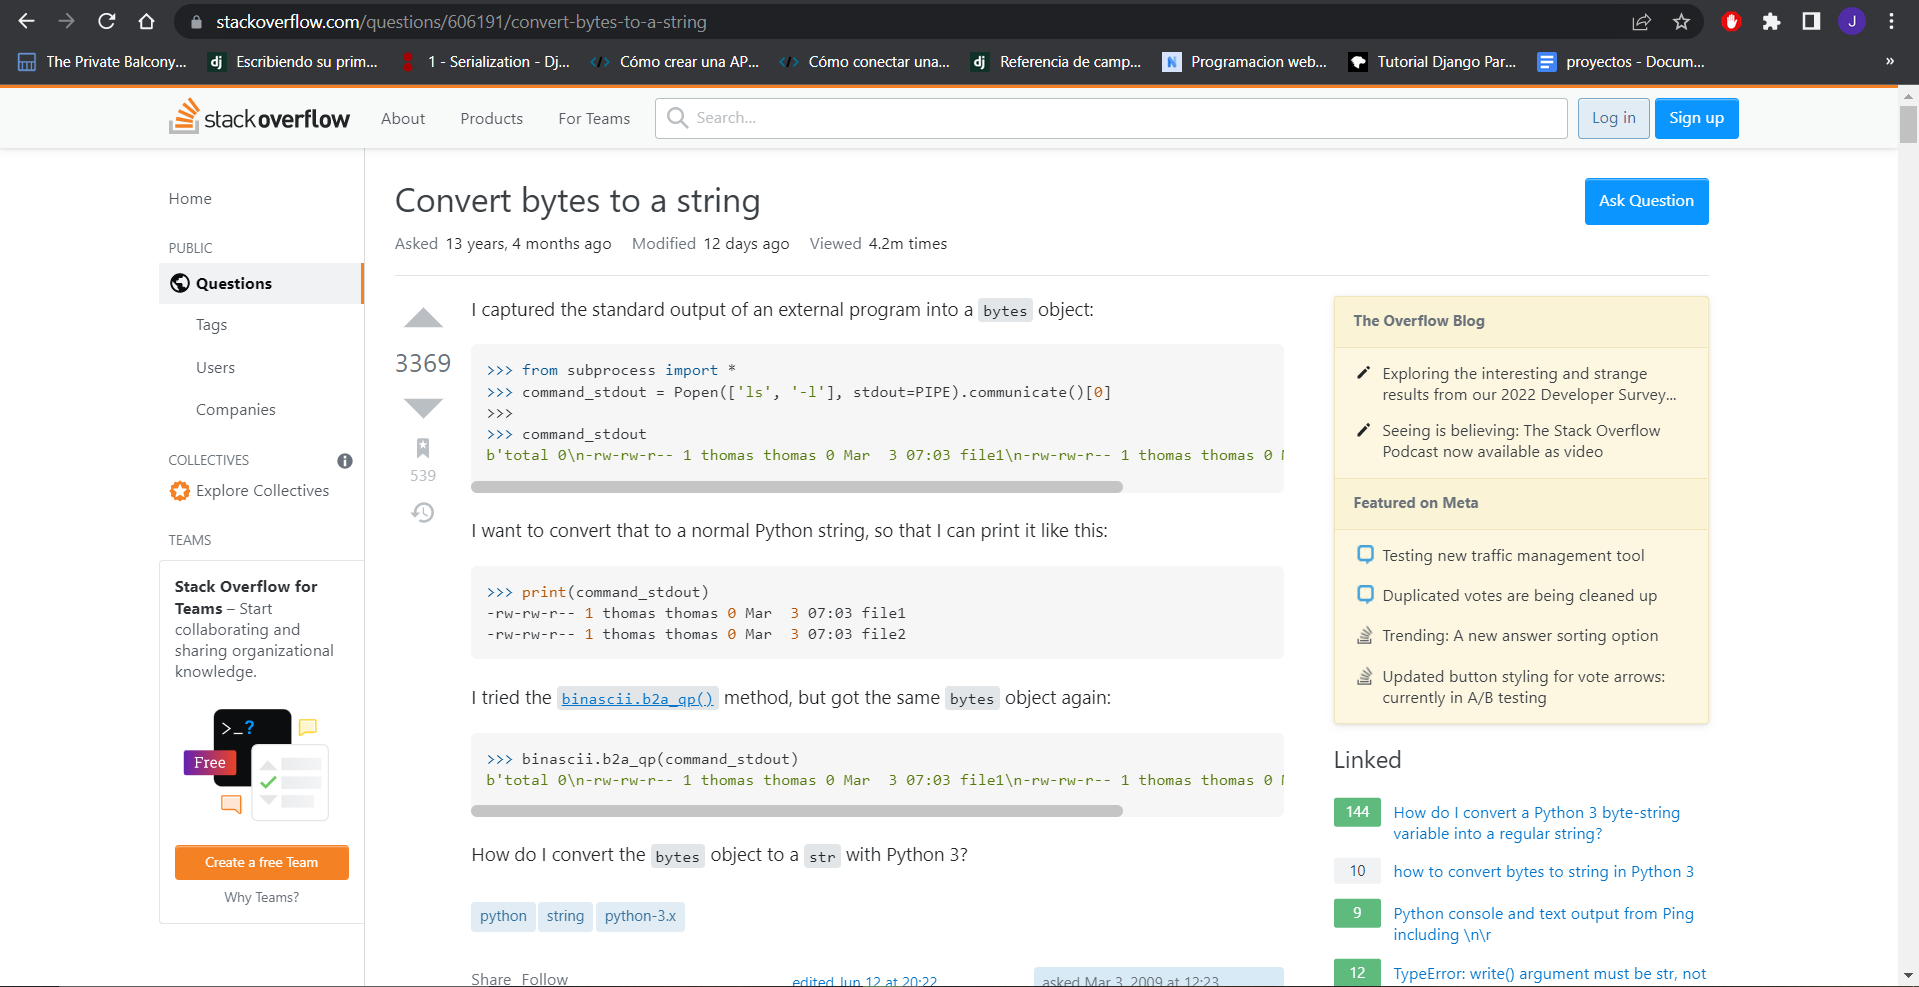
\includegraphics[bb=0 0 800 600, width=12cm, keepaspectratio]{img/stack3}
    \caption{Pregunta de ejemplo de Stack Overflow}
    \label{figura:stack3}
 \end{figure}
 
 
Antes de continuar con el comando final crearemos, dentro del directorio de nuestra herramienta, el directorio donde se guardaran los fragmentos de código analizados de Stack Overflow con el comando:

\begin{verbatim}
mkdir /test_directory
\end{verbatim}

Con esto ya solo nos queda copiar la URL y ejecutar el comando dentro del directorio local de nuestra herramienta de esta manera:

\begin{verbatim}
	python3 pycerfl.py stack <url_stack>
\end{verbatim}

Al ejecutarlo nos da una respuesta como la de la figura \ref{figura:stack4}.

\begin{figure}
	\centering
    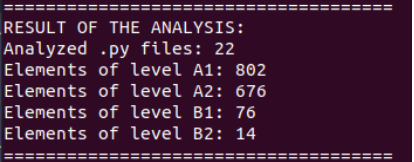
\includegraphics[width=0.5\textwidth]{img/stack4}
    \caption{Resultado de análisis de Stack Overflow}
    \label{figura:stack4}
\end{figure}

\section{Manual de análisis Pull Request}

Al igual que en la sección anterior con stack Overflow, ahora, pasamos a explicar el procedimiento a seguir para el análisis de los Pull Request.

Para ello lo primero que se debe hacer es entrar en la página web principal de GitHub y acceder a ella con nuestra cuenta:

\begin{verbatim}
	https://github.com/
\end{verbatim}

Una vez que entremos nos aparecerá una página como la de la figura \ref{figura:git1}, donde pincharemos en el botón de arriba y ligeramente a la izquierda llamado `Explore'.

\begin{figure}
    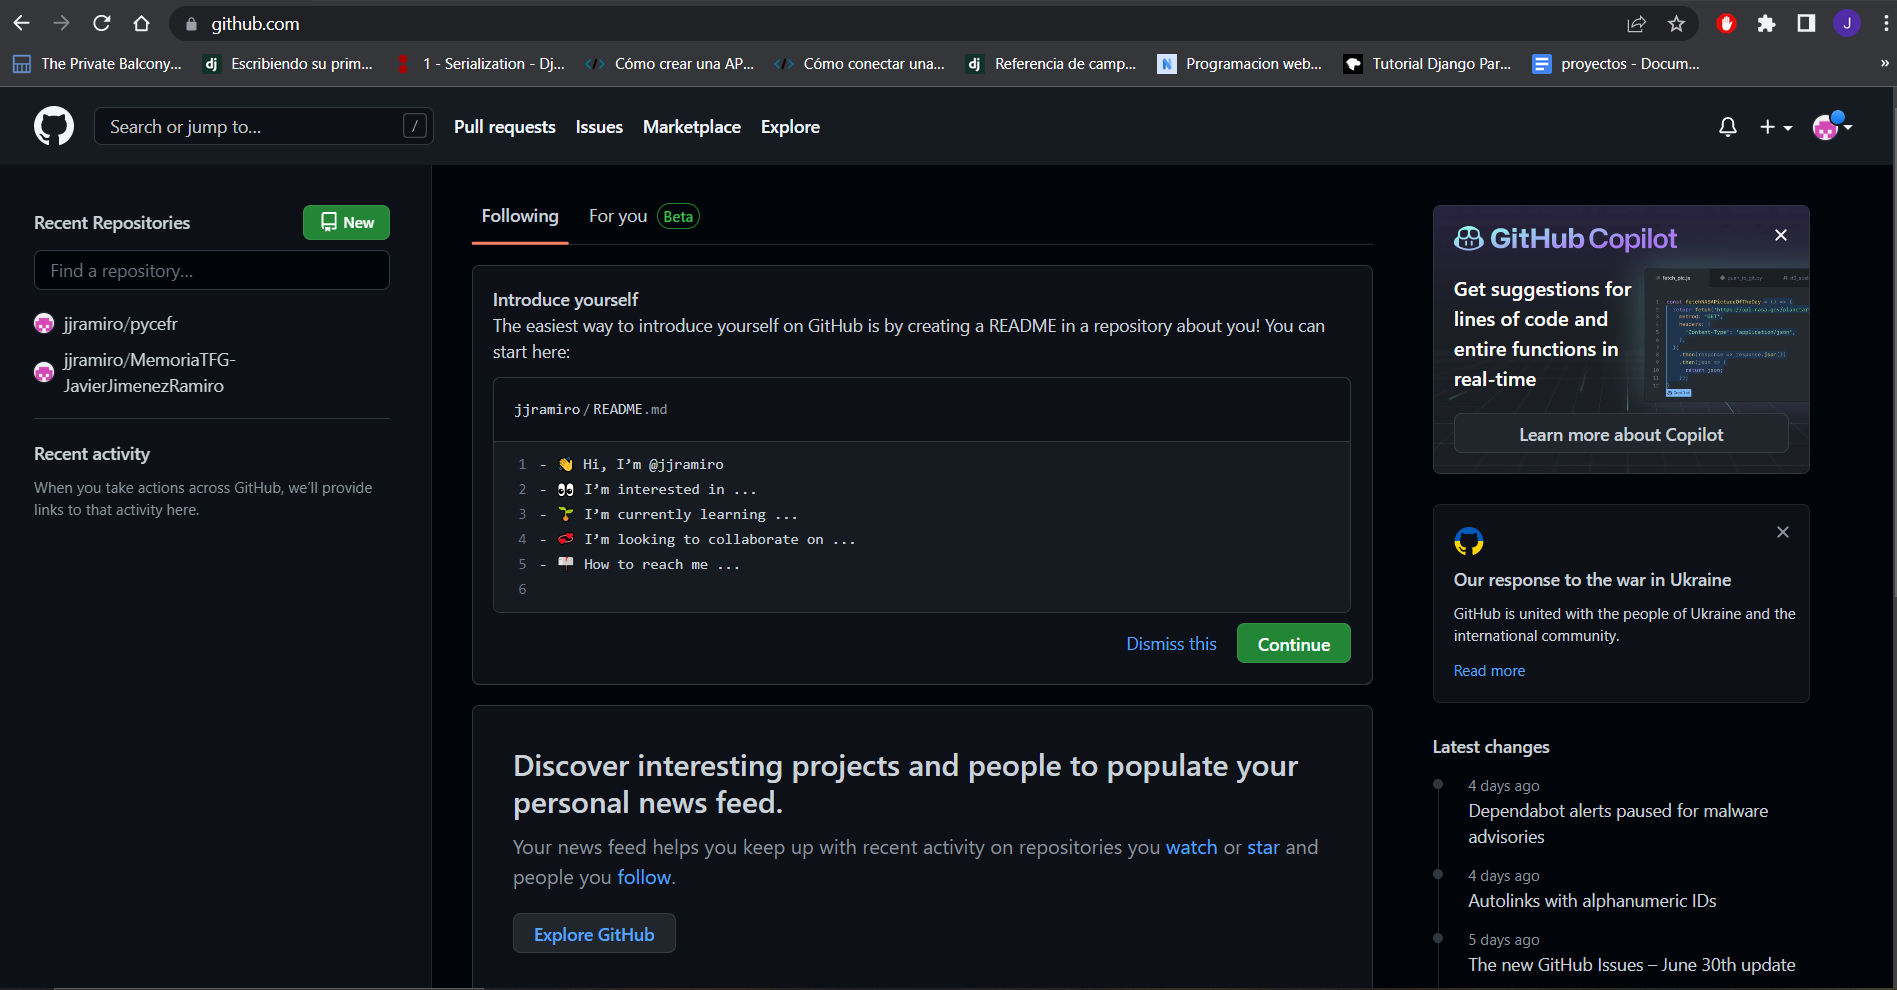
\includegraphics[bb=0 0 800 600, width=12cm, keepaspectratio]{img/git1}
    \caption{Página principal de GitHub}
    \label{figura:git1}
 \end{figure}
 
Aquí se pueden ver varios apartados dentro de `Explore'. En estos apartados pincharemos en `topic' y nos aparecerá algo parecido a la figura \ref{figura:git2}. Dentro de topic buscaremos el tema que nos interesa para el buen funcionamiento de nuestra herramienta que en nuestro caso es `Python' y pincharemos en el.

\begin{figure}
    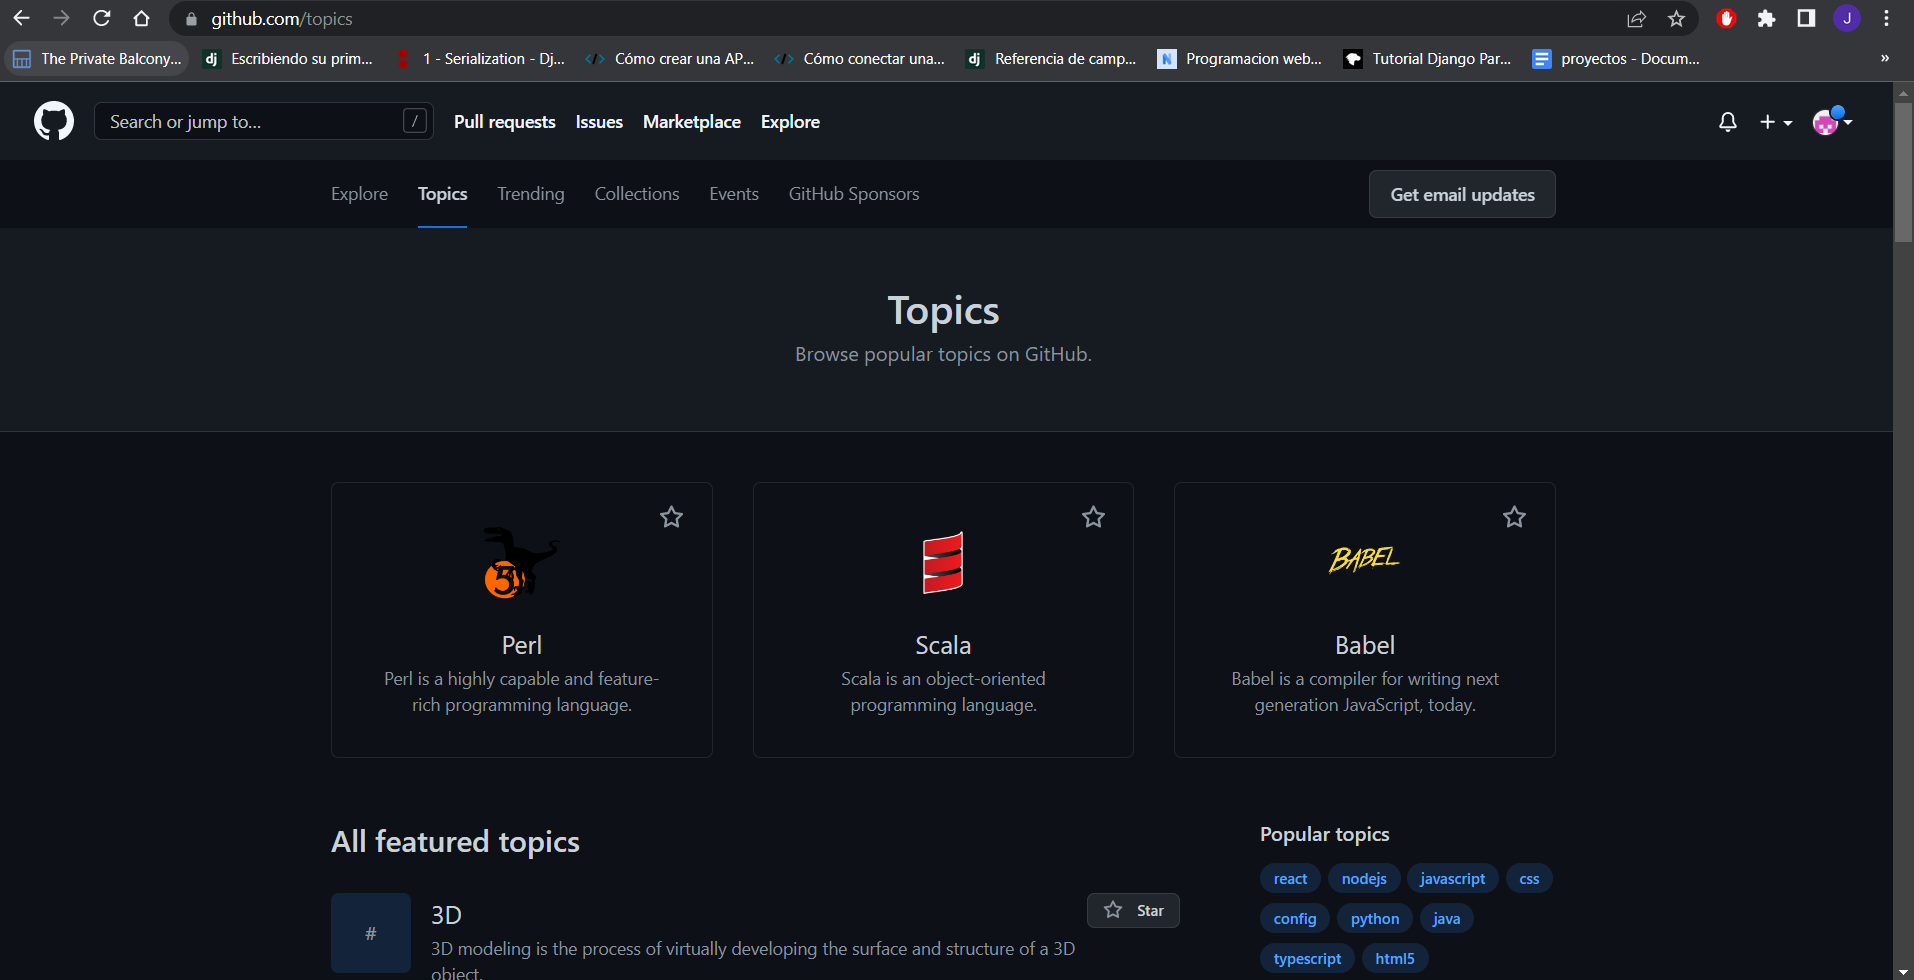
\includegraphics[bb=0 0 800 600, width=12cm, keepaspectratio]{img/git2}
    \caption{Página `topic' de GitHub}
    \label{figura:git2}
 \end{figure}
 
Ahora, como podemos ver en la figura \ref{figura:git3}, pincharemos en la parte de `language' y seleccionaremos Python, esto lo hacemos para asegurarnos de que los Pull Request son de este lenguaje y así nuestro análisis funcione correctamente.

Como resultado, se puede ver que aparecen una lista de repositorios de usuarios de GitHub y si nos fijamos bien en uno cualquiera podemos ver que tiene un botón donde se lee `pull request'. 

\begin{figure}
    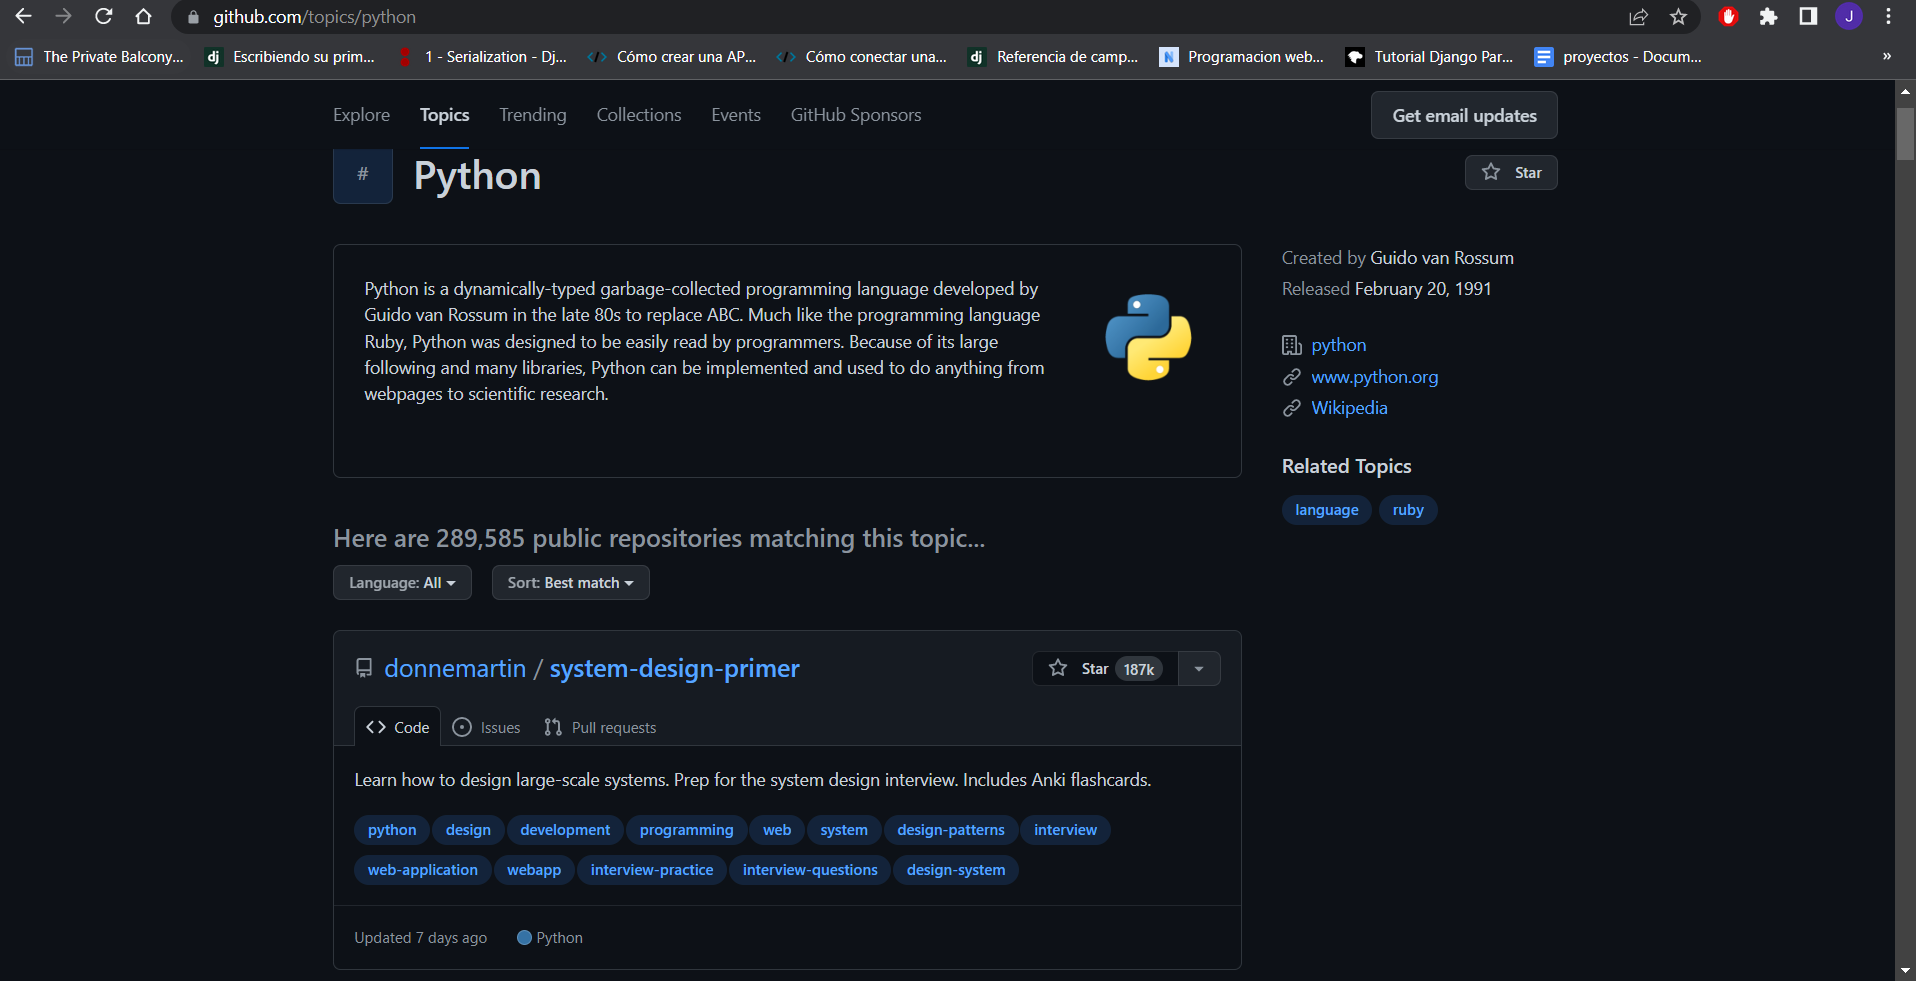
\includegraphics[bb=0 0 800 600, width=12cm, keepaspectratio]{img/git3}
    \caption{Página `topic' de Python en GitHub}
    \label{figura:git3}
 \end{figure}
 
Eligiendo cualquiera de estos proyectos y pinchando en el botón mencionado en el párrafo anterior nos aparece lo que vemos en la figura \ref{figura:git4}.

\begin{figure}
    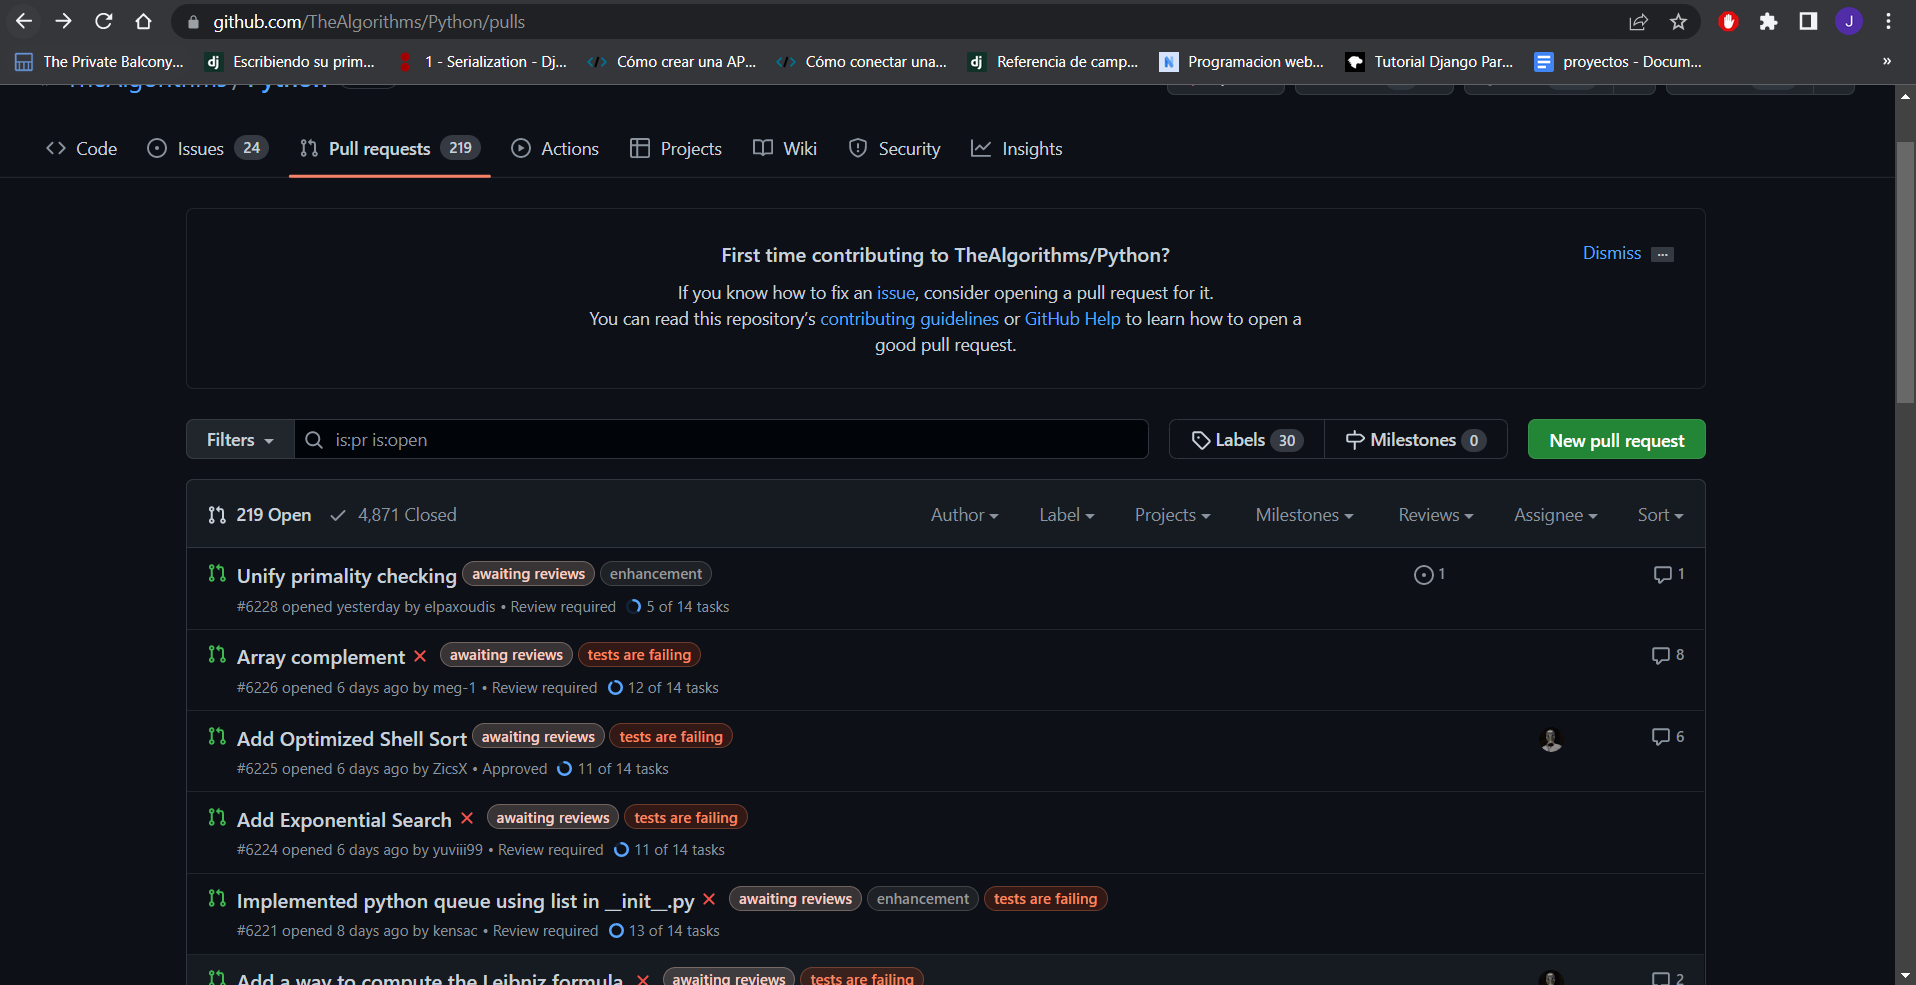
\includegraphics[bb=0 0 800 600, width=12cm, keepaspectratio]{img/git4}
    \caption{Página `pull request' de un repositorio en GitHub}
    \label{figura:git4}
 \end{figure}
 
Antes de continuar con el comando final crearemos, dentro del directorio de nuestra herramienta, el directorio donde se guardaran los fragmentos de código analizados de los Pull Request con el comando:

\begin{verbatim}
mkdir /test_directory
\end{verbatim}
 
Por último, solo quedaría elegir cualquiera de estos `pull', pinchar en el y copiar la URL resultante para poder ejecutar dentro del directorio de Pycefrl el siguiente comando:

\begin{verbatim}
python3 pycefrl.py pull <url_pull_request>
\end{verbatim}

Al ejecutarlo nos debe dar una respuesta, al igual que con Stack Overflow, parecida a la figura \ref{figura:stack4}. 

%%%%%%%%%%%%%%%%%%%%%%%%%%%%%%%%%%%%%%%%%%%%%%%%%%%%%%%%%%%%%%%%%%%%%%%%%%%%%%%%
%%%%%%%%%%%%%%%%%%%%%%%%%%%%%%%%%%%%%%%%%%%%%%%%%%%%%%%%%%%%%%%%%%%%%%%%%%%%%%%%
% EXPERIMENTOS Y VALIDACIÓN %
%%%%%%%%%%%%%%%%%%%%%%%%%%%%%%%%%%%%%%%%%%%%%%%%%%%%%%%%%%%%%%%%%%%%%%%%%%%%%%%%

\cleardoublepage
\chapter{Experimentos y validación}

En este punto ya sabemos como esta desarrollada la herramienta y el correcto modo de uso ejemplificado para conseguir un resultado favorable. Por lo tanto en este capítulo se recoge todas las pruebas y cálculos que se han hecho para aproximar el porcentaje de acierto de la herramienta en los casos de Stack Overflow y Pull Request. 

Para estos dos casos se han probado, siguiendo el método explicado en el capítulo 5, cien URLs distintas para cada uno, es decir, doscientas URLs en total.

En el caso de Stack Overflow, cada una de las URL trata de una pregunta distinta, se han intentado evitar todas las preguntas que no tuvieran respuestas o bien que, aun filtrando en la página de preguntas por lenguaje Python, no contuvieran este lenguaje.

Por otro lado en los Pull Requests, se han intentado evitar aquellos que únicamente tenían fragmentos de código sin acabar, como por ejemplo un trozo de una función, o aquellos que directamente estuvieran mal escritos. También se han evitado todos aquellos que no contuvieran, aun filtrando por Python, este lenguaje.

En cuanto a los resultados, en el caso de Stack Overflow, se ha calculado el porcentaje de acierto de cada una de las URL y después el porcentaje total juntando todos los individuales sobre cien haciendo la media. Este calculo se ha hecho dividiendo todos aquellos fragmentos analizados correctamente frente a todos los fragmentos que han pasado el filtro correctamente, después, este resultado se ha multiplicado por 100 para sacar el porcentaje. En el caso de los Pull Request, se han sumado todas aquellas URL que sus fragmentos se han analizado correctamente, que al ser 100 las totales, nos daba directamente el porcentaje de acierto.

A continuación muestro en las figuras \ref{figura:stack5}, \ref{figura:stack6}, \ref{figura:stack7}, \ref{figura:stack8}, \ref{figura:stack9}, \ref{figura:stack10}, \ref{figura:stack11}, \ref{figura:stack12}, \ref{figura:stack13}, \ref{figura:stack14}, \ref{figura:stack15}, todas las URL de Stack Overflow seguidas de sus resultados y su porcentaje:

\begin{figure}
	\centering
    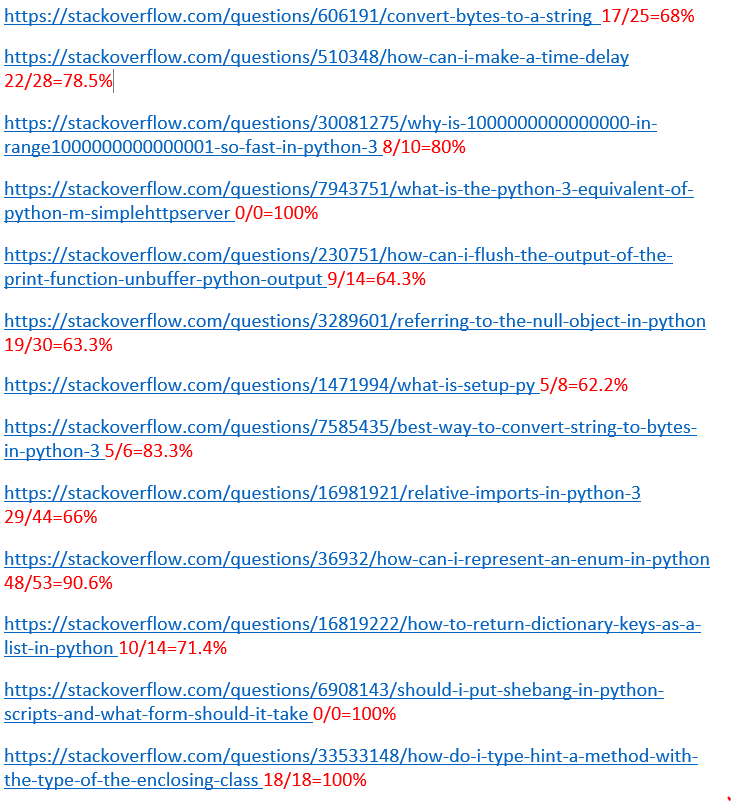
\includegraphics[width=1\textwidth]{img/stack5}
    \caption{Resultados Stack Overflow (1)}
    \label{figura:stack5}
 \end{figure}
 
\begin{figure}
	\centering
    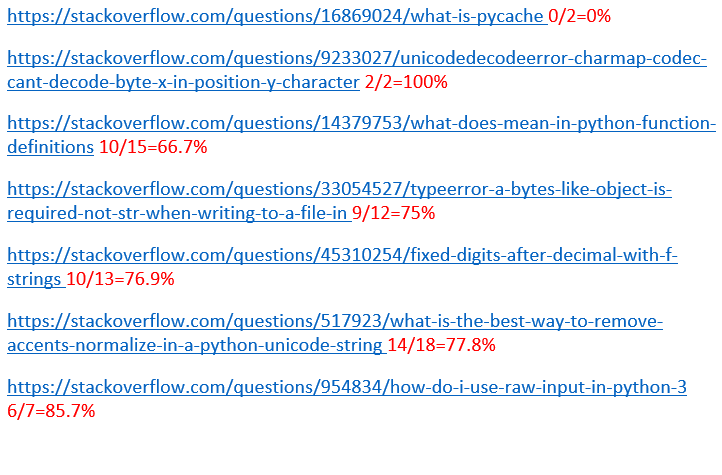
\includegraphics[width=1\textwidth]{img/stack6}
    \caption{Resultados Stack Overflow (2)}
    \label{figura:stack6}
 \end{figure}
 
\begin{figure}
	\centering
    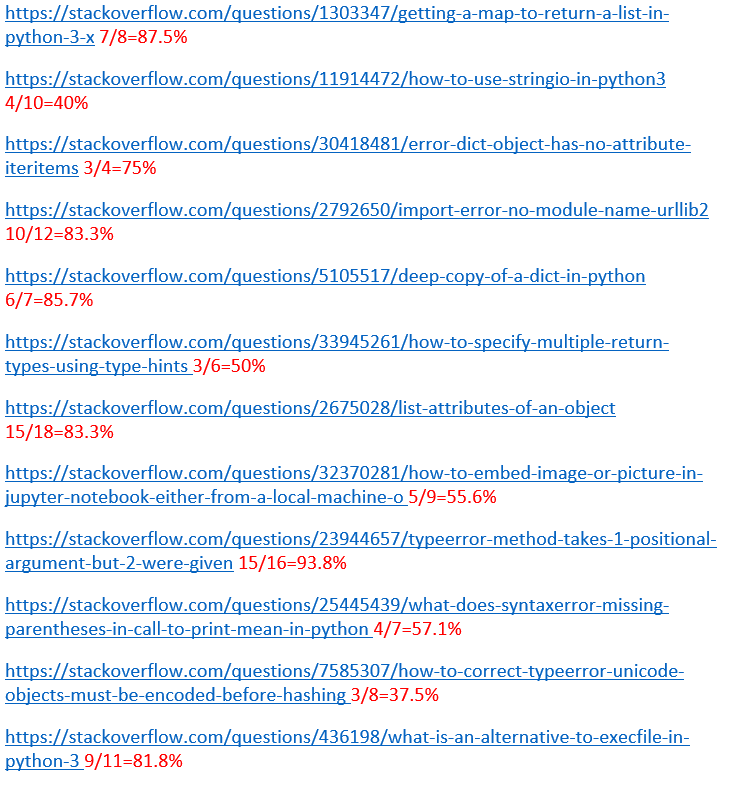
\includegraphics[width=1\textwidth]{img/stack7}
    \caption{Resultados Stack Overflow (3)}
    \label{figura:stack7}
 \end{figure}
 
\begin{figure}
	\centering
    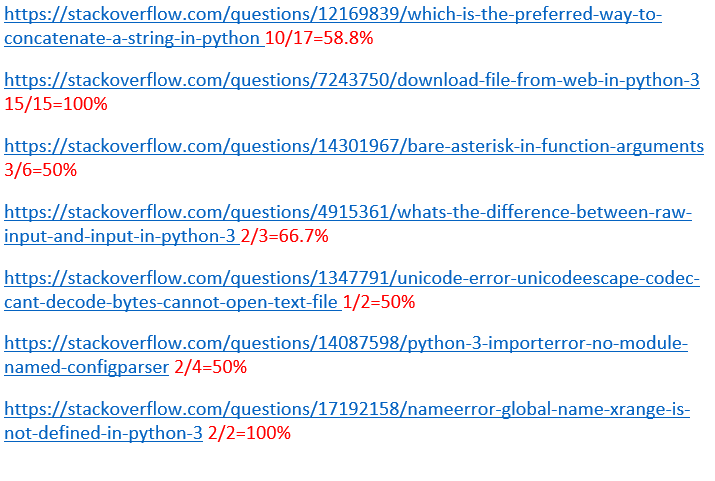
\includegraphics[width=1\textwidth]{img/stack8}
    \caption{Resultados Stack Overflow (4)}
    \label{figura:stack8}
 \end{figure}
 
\begin{figure}
	\centering
    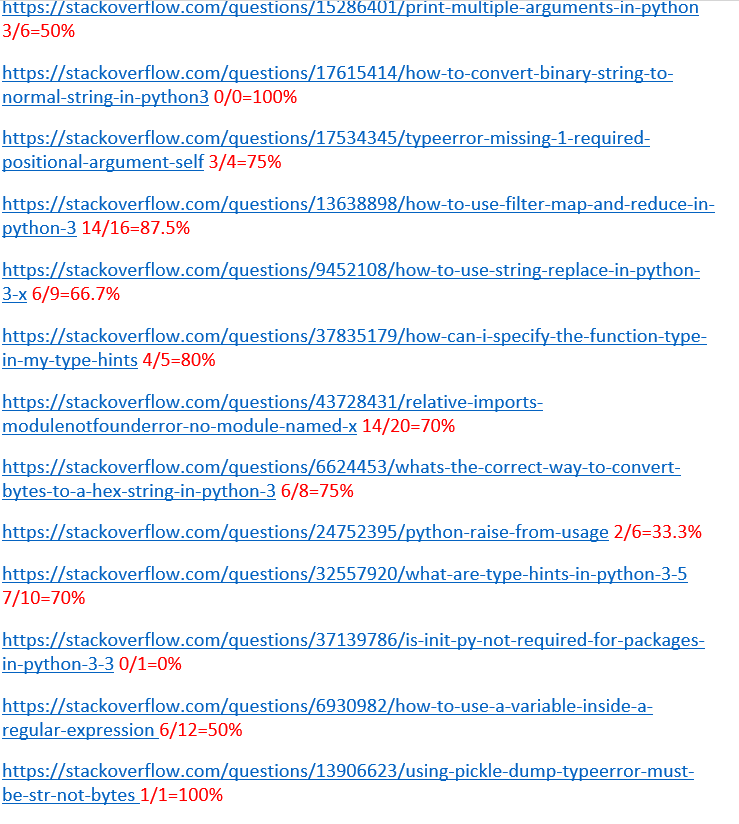
\includegraphics[width=1\textwidth]{img/stack9}
    \caption{Resultados Stack Overflow (5)}
    \label{figura:stack9}
 \end{figure}
 
\begin{figure}
	\centering
    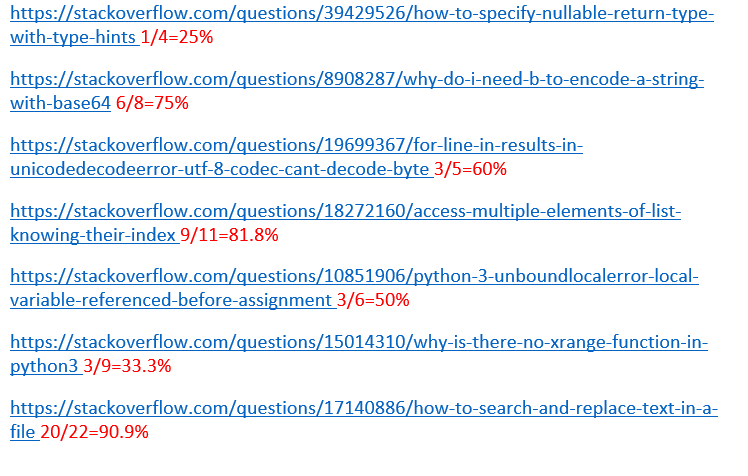
\includegraphics[width=1\textwidth]{img/stack10}
    \caption{Resultados Stack Overflow (6)}
    \label{figura:stack10}
 \end{figure}
 
\begin{figure}
	\centering
    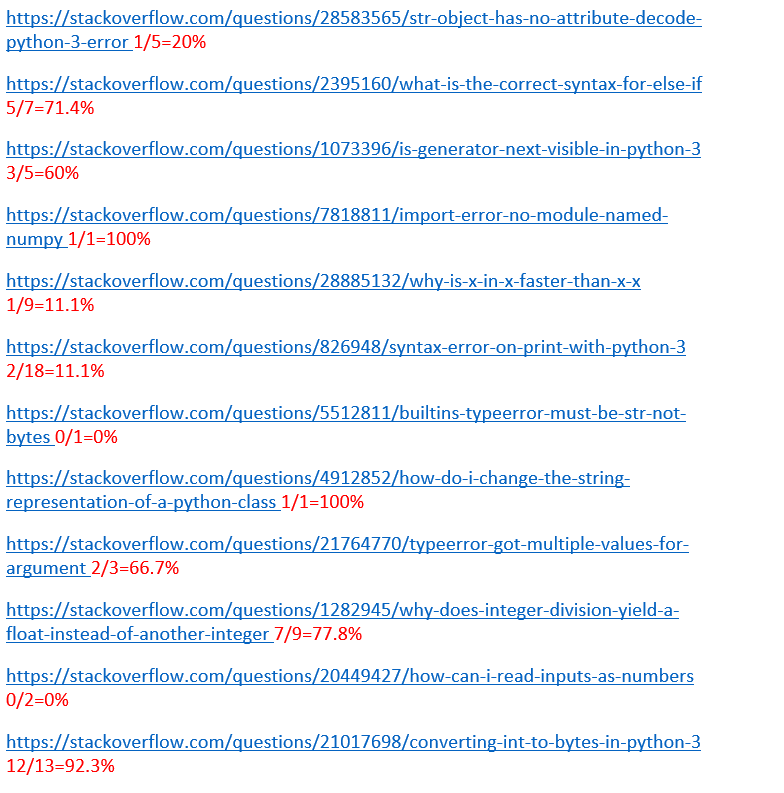
\includegraphics[width=1\textwidth]{img/stack11}
    \caption{Resultados Stack Overflow (7)}
    \label{figura:stack11}
 \end{figure}
 
\begin{figure}
	\centering
    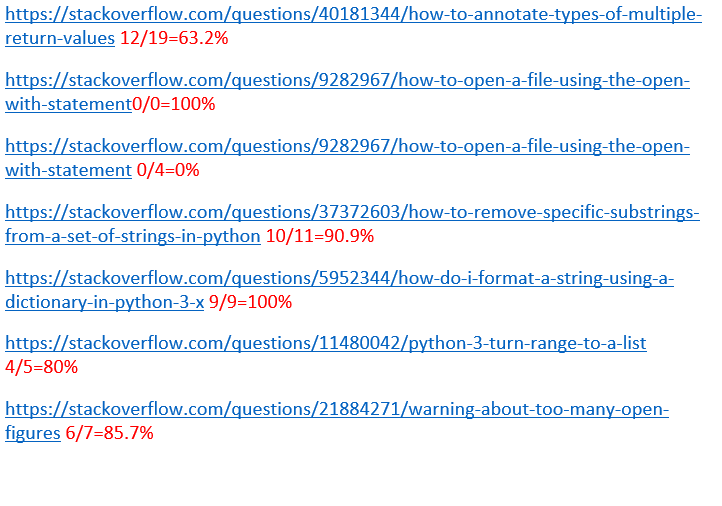
\includegraphics[width=1\textwidth]{img/stack12}
    \caption{Resultados Stack Overflow (8)}
    \label{figura:stack12}
 \end{figure}
 
\begin{figure}
	\centering
    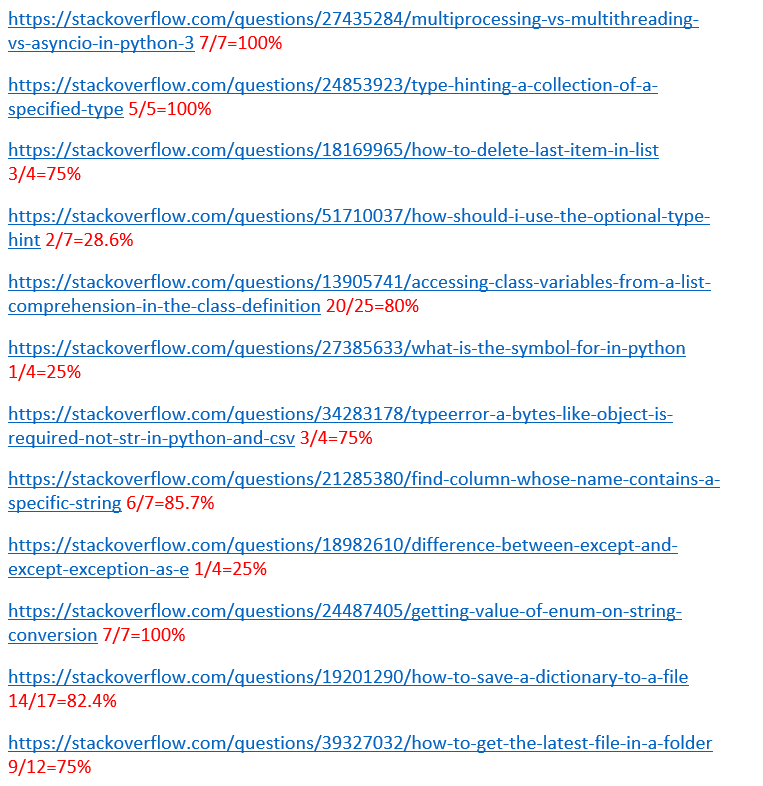
\includegraphics[width=1\textwidth]{img/stack13}
    \caption{Resultados Stack Overflow (9)}
    \label{figura:stack13}
 \end{figure}
 
\begin{figure}
	\centering
    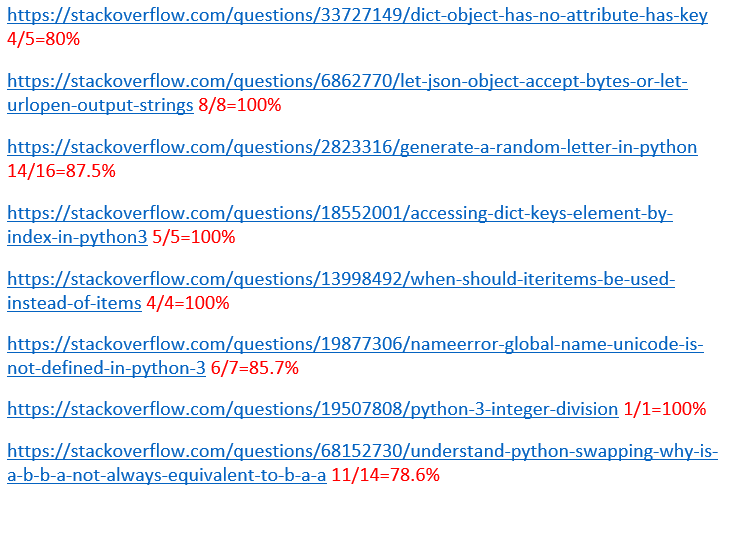
\includegraphics[width=1\textwidth]{img/stack14}
    \caption{Resultados Stack Overflow (10)}
    \label{figura:stack14}
 \end{figure}
 
\begin{figure}
	\centering
    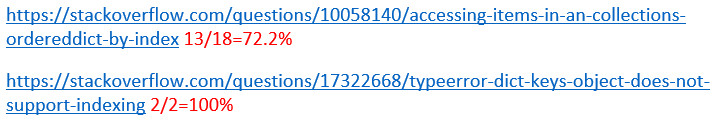
\includegraphics[width=1\textwidth]{img/stack15}
    \caption{Resultados Stack Overflow (11)}
    \label{figura:stack15}
 \end{figure}

Por último, teniendo en cuenta todos los resultados mostrados y haciendo el porcentaje final, nos da como porcentaje de acierto completo un 70.4.

A continuación muestro en las figuras \ref{figura:git5}, \ref{figura:git6}, \ref{figura:git7}, \ref{figura:git8}, \ref{figura:git9}, \ref{figura:git10}, \ref{figura:git11}, todas las URL de los Pull Request seguidas de si se han analizado (y) correctamente o no(n):

\begin{figure}
	\centering
    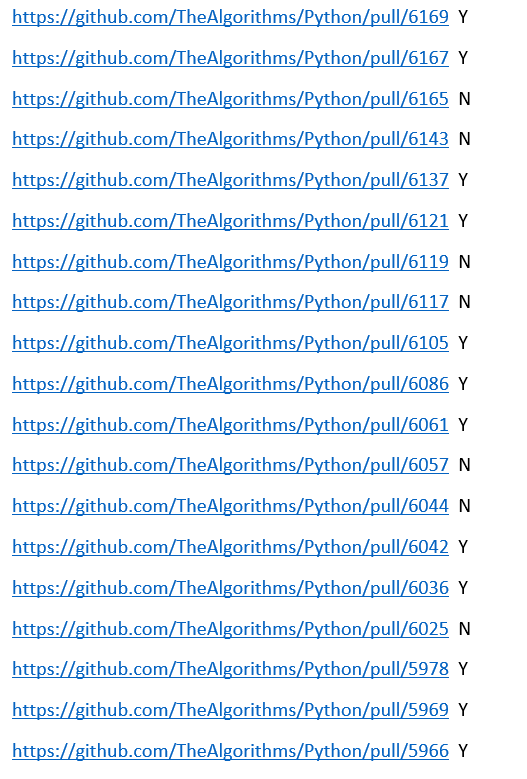
\includegraphics[width=0.7\textwidth]{img/git5}
    \caption{Resultados Pull Request (1)}
    \label{figura:git5}
 \end{figure}
 
\begin{figure}
	\centering
    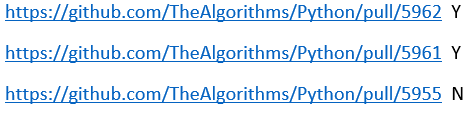
\includegraphics[width=0.7\textwidth]{img/git6}
    \caption{Resultados Pull Request (2)}
    \label{figura:git6}
 \end{figure}
 
\begin{figure}
	\centering
    
\includegraphics[width=0.7\textwidth]{img/git7}
    \caption{Resultados Pull Request (3)}
    \label{figura:git7}
 \end{figure}
 
\begin{figure}
	\centering
    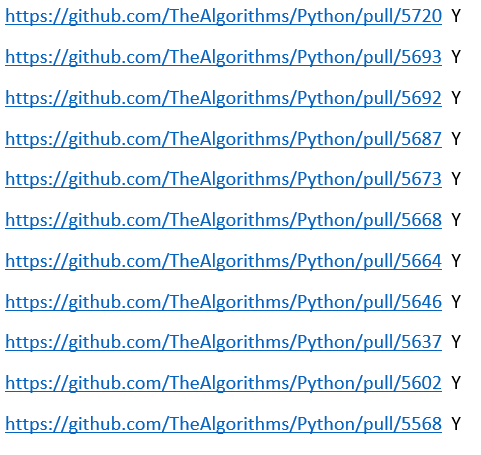
\includegraphics[width=0.7\textwidth]{img/git8}
    \caption{Resultados Pull Request (4)}
    \label{figura:git8}
 \end{figure}
 
\begin{figure}
	\centering
    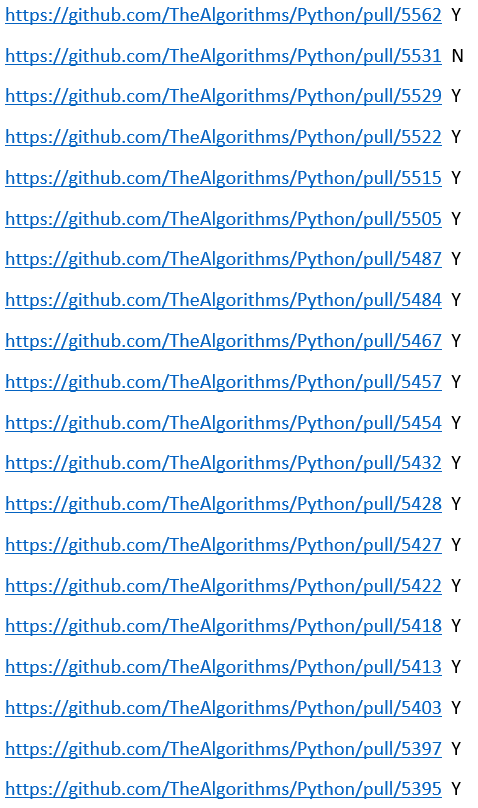
\includegraphics[width=0.7\textwidth]{img/git9}
    \caption{Resultados Pull Request (5)}
    \label{figura:git9}
 \end{figure}
 
\begin{figure}
	\centering
    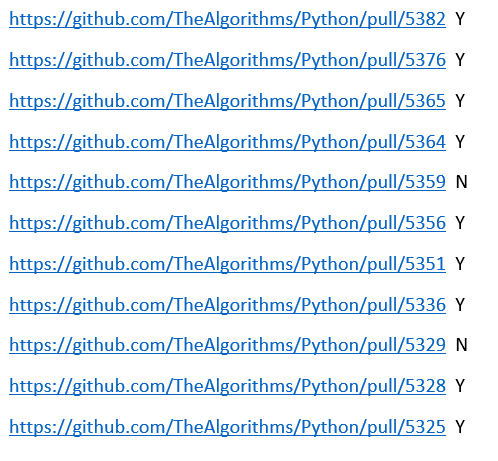
\includegraphics[width=0.7\textwidth]{img/git10}
    \caption{Resultados Pull Request (6)}
    \label{figura:git10}
 \end{figure}
 
\begin{figure}
	\centering
    
\includegraphics[width=0.7\textwidth]{img/git11}
    \caption{Resultados Pull Request (7)}
    \label{figura:git11}
 \end{figure}
 
Juntando todos los aciertos dentro de los Pull Request llegamos a un resultado de aciertos en total de ochenta y seis sobre cien, es decir, un 86 por ciento.


%%%%%%%%%%%%%%%%%%%%%%%%%%%%%%%%%%%%%%%%%%%%%%%%%%%%%%%%%%%%%%%%%%%%%%%%%%%%%%%%
%%%%%%%%%%%%%%%%%%%%%%%%%%%%%%%%%%%%%%%%%%%%%%%%%%%%%%%%%%%%%%%%%%%%%%%%%%%%%%%%
% CONCLUSIONES %
%%%%%%%%%%%%%%%%%%%%%%%%%%%%%%%%%%%%%%%%%%%%%%%%%%%%%%%%%%%%%%%%%%%%%%%%%%%%%%%%

\cleardoublepage
\chapter{Conclusiones}
\label{chap:conclusiones}


\section{Consecución de objetivos}
\label{sec:consecucion-objetivos}

Como se comentó en el capítulo 2, el objetivo de este proyecto era el de ampliar la herramienta ya existente y creada por mi compañera Ana Poveda García Herrero con dos nuevas opciones de análisis, Stack overflow y Pull Request de GitHub, para poder cerciorarnos de como de bueno es un código y como de útil puede ser implementarlo en nuestros proyectos dependiendo de su nivel. Por lo tanto el objetivo general se ha cumplido.

En cuánto a los objetivos específicos, podemos observar que también han sido cumplidos aunque esta vez con complicaciones y no tan bien perfeccionados como se podría esperar.

Esto ocurre por las limitaciones propias que nos presentan estas dos opciones y que tienen una alta dificultad para solucionarlas y se podría definir como la ``libertad" que nos dan estas opciones. Esta libertad trata de que tanto en Stack Overflow como en los Pull Request de GitHub cualquier usuario puede aportar cualquier cosa, pudiendo añadir, dentro del filtrado de Python, otros lenguajes, texto plano o incluso fragmentos de código mal escritos o sin acabar.

Para este tipo de problemas lo único que tenemos como `defensa' es una excepción ya creada en la anterior versión de la herramienta.

Y aunque es cierto que, como vemos en el capítulo 6, tenemos unos resultados muy favorables y con un buen porcentaje de acierto, hay que tener en cuenta que tienen que darse las condiciones de que el lenguaje sea Python3 y que el código este bien escrito y acabado para que el análisis sea correcto. Quitando estas dificultades bastante complicadas de abordar podemos asegurar que los objetivos se han cumplido satisfactoriamente.

\section{Aplicación de lo aprendido}
\label{sec:aplicacion}

En cuanto a la aplicación de lo aprendido, considero que todas las asignaturas del grado y todos los profesores con los que he tenido oportunidad de encontrarme han aportado, directa o indirectamente, su granito de arena para hacerme llegar hasta aquí, bien sea por los conocimientos aprendidos o por la manera de enseñarme a gestionar cierto tipo de problemas con los que me he encontrado en este último año, pero sí me gustaría destacar algunas asignaturas que han sobresalido:

\begin{enumerate}
  \item \textbf{Informática 1:} Esta asignatura fue mi primer contacto con la programación y me ayudó a saber que había escogido el camino correcto y que todos los problemas son divisibles.
  \item \textbf{Informática 2:} Esta asignatura me planteo nuevos retos, me enseñó la importancia de los paquetes y de las librerías y me enseñó que el mundo de la programación es inmenso y repleto de buenas ideas.
  \item \textbf{Protocolos para la transmisión de audio y vídeo por Internet (ptavi):} Esta asignatura me ayudó a descubrir el que es mi lenguaje favorito, Python, y sus profesores me transmitieron aun más pasión por el mundo de la programación. Por ello tenía claro que mi proyecto tenía que estar orientado a Python.
  \item \textbf{Prácticas externas:} Aunque no es una asignatura como tal, el haber hecho mis prácticas con Python me ayudó a consolidar más mis conocimientos sobre el lenguaje y me hizo mucho más fácil el hecho de poder depurar errores y dejar el código todo lo limpio que supe.
\end{enumerate}


\section{Lecciones aprendidas}
\label{sec:lecciones_aprendidas}

Además de todo lo aprendido en mi paso por el grado, he aprendido lecciones muy importantes de este proyecto, las cuales son:

\begin{itemize}
	\item Este proyecto me ha ayudado a consolidar aun más los conocimientos sobre Python, sobre sus librerías y a ser algo más independiente a la hora de programar en el. Y aunque aun me queda camino por recorrer, sé que estoy en el sendero correcto.
	\item También me ha ayudado a entender mejor el funcionamiento tanto de Stack overflow como de GitHub, más concretamente los Pull Request. Ya que al tener que analizarlos y utilizarlos me he dado cuenta de todas las posibilidades que ofrecen cada una de estas webs.
	\item Otra lección aprendida es el uso de \LaTeX. Me ha hecho darme cuenta de lo útil que puede llegar a ser este lenguaje para la creación y edición de proyectos y lo cómodo que resulta trabajar con el.
	\item Como última lección destacable añadiría la gestión y organización de un proyecto algo más grande. La realización de este proyecto me ha ayudado a saber organizar mejor este tipo de proyectos más prolongados en el tiempo. 
\end{itemize}

\section{Trabajos futuros}
\label{sec:trabajos_futuros}

La ampliación de esta herramienta y todo lo desarrollado en este proyecto es solo una pequeña mejora de todo lo que se podría añadir. Hay un gran abanico de mejoras y funcionalidades que se podrían implementar por lo que aquí dejo algunas ideas:

\begin{itemize}
	\item Se podría mejorar con un analizador propio la cantidad de lenguajes a analizar añadiendo por ejemplo Python2 u otro tipo de lenguajes.
	\item Se pueden añadir más filtros y aun más controles de errores para mejorar el porcentaje de acierto de las nuevas opciones.
	\item Se pueden añadir nuevas funcionalidades para que en el resultado no solo aparezca tu nivel si no también como mejorarlo y que elementos implementar para elevar el nivel de tu proyecto.
\end{itemize}


%%%%%%%%%%%%%%%%%%%%%%%%%%%%%%%%%%%%%%%%%%%%%%%%%%%%%%%%%%%%%%%%%%%%%%%%%%%%%%%%
%%%%%%%%%%%%%%%%%%%%%%%%%%%%%%%%%%%%%%%%%%%%%%%%%%%%%%%%%%%%%%%%%%%%%%%%%%%%%%%%
% APÉNDICE(S) %
%%%%%%%%%%%%%%%%%%%%%%%%%%%%%%%%%%%%%%%%%%%%%%%%%%%%%%%%%%%%%%%%%%%%%%%%%%%%%%%%

%\cleardoublepage
%\appendix
%\chapter{Manual de usuario}
%\label{app:manual}

%Esto es un apéndice.
%Si has creado una aplicación, siempre viene bien %tener un manual de usuario.
%Pues ponlo aquí.

%%%%%%%%%%%%%%%%%%%%%%%%%%%%%%%%%%%%%%%%%%%%%%%%%%%%%%%%%%%%%%%%%%%%%%%%%%%%%%%%
%%%%%%%%%%%%%%%%%%%%%%%%%%%%%%%%%%%%%%%%%%%%%%%%%%%%%%%%%%%%%%%%%%%%%%%%%%%%%%%%
% BIBLIOGRAFIA %
%%%%%%%%%%%%%%%%%%%%%%%%%%%%%%%%%%%%%%%%%%%%%%%%%%%%%%%%%%%%%%%%%%%%%%%%%%%%%%%%

\cleardoublepage

% Las siguientes dos instrucciones es todo lo que necesitas
% para incluir las citas en la memoria
\bibliographystyle{abbrv}
\bibliography{memoria}  % memoria.bib es el nombre del fichero que contiene
% las referencias bibliográficas. Abre ese fichero y mira el formato que tiene,
% que se conoce como BibTeX. Hay muchos sitios que exportan referencias en
% formato BibTeX. Prueba a buscar en http://scholar.google.com por referencias
% y verás que lo puedes hacer de manera sencilla.
% Más información: 
% http://texblog.org/2014/04/22/using-google-scholar-to-download-bibtex-citations/

\end{document}
